\documentclass[a4paper,12pt]{report}

%\usepackage{caption}
\usepackage{subcaption}

\newcommand*{\tabbox}[2][t]{%
        \vspace{0pt}\parbox[#1][3.7\baselineskip]{1cm}{\strut#2\strut}}

\usepackage{amsmath}
\usepackage{amsfonts}

\usepackage{tikz}
\usetikzlibrary{intersections,positioning,calc,arrows,shapes,
                decorations.pathreplacing,spy,automata}

\usepackage{pgfplots}
%\pgfplotsset{compat=1.7}

\usepackage{cite}

\usepackage[ruled]{algorithm2e}

\usepackage{paralist}

\usepackage{url}

\usepackage{verbatim}
\usepackage{chngcntr}
\counterwithin{figure}{chapter}
\counterwithin{equation}{chapter}
\counterwithin{table}{chapter}
\counterwithin{algocf}{chapter}

\DeclareMathOperator*{\argmin}{arg\,min}
\DeclareMathOperator*{\argmax}{arg\,max}

\makeatletter
\tikzset{circle split part fill/.style  args={#1,#2}{%
alias=tmp@name, % Jake's idea !!
postaction={%
insert path={
\pgfextra{
\pgfpointdiff{\pgfpointanchor{\pgf@node@name}{center}}
{\pgfpointanchor{\pgf@node@name}{east}}
\pgfmathsetmacro\insiderad{\pgf@x}
\fill[#1] (\pgf@node@name.base) ([xshift=-\pgflinewidth]\pgf@node@name.east) arc
          (0:180:\insiderad-\pgflinewidth)--cycle;
\fill[#2] (\pgf@node@name.base) ([xshift=\pgflinewidth]\pgf@node@name.west) arc
          (180:360:\insiderad-\pgflinewidth)--cycle;
}}}}}
\makeatother

\begin{document}

\title{Fast Solver of Closely Related Quadratic Programming
       Problems.}
\date{June 1, 2013}
\author{Andreas Halle}
\maketitle
\thispagestyle{empty}
\newpage

\thispagestyle{empty}
\begin{abstract}
Goodtech and MathConsult have developed a tool called PROMAPS.
It calculates the power delivery as a function of demand, and the probability
for undelivered energy for each load branch in the system, and in the
system as a whole. This problem is formulated as several closely related 
quadratic programming (QP) problems, whose only difference is in the column
bounds. A major part of the bottleneck of PROMAPS, has been found to be
calls to a QP solver. The aim of this thesis is to develop a fast solver
with the characteristics of these QP problems. The characteristics of the
QP problems suggest that methods based upon linear programming (LP) are
suited for solving them. In this thesis, we present an iterative QP solver
using methods based upon linear programming. We also present a tree structured
method that reduces the number of calls to a QP solver by a significant amount.

%Goodtech and MathConsult have developed tools to compute the reliability of
%delivery in a masked network where every link has an error rate. 
%This method is based on reliability theory to find actual error cases for
%further analysis, and optimization theory to compute an optimal delivery
%through the network for every error case.
%The optimization problems are formulated as Quadratic Programming (QP)
%problems. For each problem, Goodtech wants to solve a number of closely
%related QP problems, with only minor changes in the column bounds.
%The aim of this thesis is to develop a solver for effectively
%solving the formulated QP problems. The way the QP problems are formulated
%suggests that methods based upon linear programming (LP) are suited
%for solving them. 
%Because the number of possible error cases increases rapidly as the size of the
%network increases, it is crucial that every error case is analyzed very
%quickly.
%The aim is to develop a solver for effectively solving problems
%\begin{inparaenum}
%  \item with a problem size of 100 to 2000 variables;
%  \item with sparse matrices;
%  \item with positive-semidefinite quadratic terms in the objective function;
%        and
%  \item where the QP problem shall be solved many times with small variations
%        in the constraints.
%\end{inparaenum}
\end{abstract}
\newpage

%\end{@twocolumnfalse}
%]
%{
%  \renewcommand{\thefootnote}%
%    {\fnsymbol{footnote}}
%  \footnotetext[1]{University of Bergen, Department of Informatics, P.O.Box 7803, N-5020 Bergen, Norway}
%}
\setcounter{page}{3}
\tableofcontents
\newpage

\chapter{Introduction}
\label{ch:intro}
As electrical transmission systems increase in complexity, it becomes
more difficult to understand how different components in the system interact.
We often aim to increase the utilization of such systems, and with that comes
the need for good planning and operational tools.
The Transmission System Operator (TSO) is faced
with increasing requirements regarding the reliability of load
delivery, and the cost of not delivering agreed energy can be
substantial.
The need for tools to assist the TSO in analyses that can help prevent
unreliable networks is important.
Digernes et al. \cite{digernes} state:
%In \cite{digernes}, the authors state:
\begin{quote}
It is of utmost importance for the TSO to be able to perform detailed and
accurate reliability analyses; for the daily operation as well as for
future planning (comparison of reinforcement alternatives etc.). By
including power flow considerations in the calculations, the operator is
able to plan where to locate the spinning reserves to maximize the load
delivery reliability. Reliability analyses are also important for system
planning, for analyzing different alternatives for network reinforcement's
[sic] etc.\cite{digernes}
\end{quote}

Goodtech and MathConsult have developed a tool called PROMAPS
(Probability Methods Applied to Power Systems). It calculates the power
delivery as a function of demand, and the probability for undelivered
energy for each load branch in the system, and in the system as a whole.
According to Svendsen et al. \cite{trond}, a typical calculation sequence
in PROMAPS includes the following main functions:
%A typical calculation sequence in PROMAPS includes the following main
%functions\cite{trond}:
\begin{enumerate}
\item Creation of branch reliability models based on unit Markov models and
      composition and aggregation of states.
\item Selection of a subset of states containing all grid reliability states
      with a significant reliability.
\item Calculation of maximum power delivery capacity for each of the
      significant grid reliability states based on an objective function with
      constraints.
\item Calculation of expected power shortage and creation of delivery
      reliability models based on the operations composition and aggregation.
\item Calculation of delivery probability, mean visiting duration and visiting
      frequency for functioning and failed delivery states.
\item Post calculation of various auxiliary variables including economic data.
\end{enumerate}
Among these six functions, the third main function has been identified as the
most time-consuming. A major part of the third main function is a call to a
QP solver\cite{trond}.

The maximum power
supply can be calculated by an objective function that represents the power
delivery profit. A typical objective function is
\begin{equation}
f(x) = x^T \Phi D x + (g-c)^T x, \label{eq:goodtech}
\end{equation}
where $f(x)$ is the objective value ($E/s$) as a function of $x$, $x$ is the
branch power vector ($W$), $g$ is a vector containing specific power
generation costs ($E/J$), $\Phi$ is a diagonal matrix representing power loss
($1/W$), $D$ is a diagonal matrix containing specific power transmission costs
($E/J$), and $c$ is a vector containing specific power delivery price
($E/J$). The symbols in parentheses are units of measurements, where $E$
denotes the monetary unit, $J$ denotes joule and $W$ denotes
watt\cite{digernes}.

We simplify (\ref{eq:goodtech}) to
\begin{equation}
    f(x) = x^T H x + b^T x, \label{eq:obj}
\end{equation}
where $H = \Phi D$ is a diagonal matrix that represents quadratic cost terms
($E/(W^2 s)$) and $b = g - c$ is a vector that represents linear cost terms
($E/J$) \cite{digernes}.

The maximum power delivery capacity can be defined as an optimization problem
\begin{equation}
   \min_{x} f(x)\quad\textrm{subject to}~Ax = 0,
                             ~l \leq x \leq u \label{eq:thesisqp}
\end{equation}
where $A$ is the grid configuration matrix or reduced incidence matrix, and
$l$ and $u$ are the minimum and maximum branch (lower and upper) capacity,
respectively\cite{digernes}.

If a branch with index $i$ fails, we can model it by letting
$l_i = u_i = 0$ where $l_i$ and $u_i$ denote the $i$th element of $l$ and
$u$, respectively. We refer to a branch failing as a \textit{breakdown}.
We discuss breakdowns in more detail in sections \ref{sec:instances} to
\ref{sec:subinstances} and Chapter \ref{ch:tree}.

In the next chapter, we present a brief introduction to linear and quadratic
programming.
We then move on to Chapter \ref{ch:qp} where we present some instances of the
quadratic programming problem (\ref{eq:obj}) that Goodtech have supplied.
Afterwards, in Chapter \ref{ch:slp}, we present
an iterative optimization method based on Successive Linear Programming (SLP).
Then we move on to Chapter \ref{ch:tree}, where we present methods for
eliminating unnecessary work carried out in the third main function of PROMAPS,
and thereby improving the speed in which it is performed.
We also present implementations of all the aforementioned methods in Chapter
\ref{ch:implementation}, along with
experiments and results in Chapter \ref{ch:experiments}.

%\begingroup
%\let\clearpage\relax
\chapter{Implementation}
Recall from Chapter \ref{ch:qp} that we discussed limiting the amount
of subinstances to solve. We did this by introducing a limit on the number of
simultaneous break-downs in the network by some $\beta$.
Another approach is to implement a discrete-event simulator (DES). Each event
occurs at a particular instant in time that changes the state of the system.
In this case, each event would either be a breakdown in the network, or that
a breakdown is fixed.

The difference in these two approaches are prominent, but they share the same
core, namely a QP solver. In this chapter we first discuss the implementation
of the solver declared in Chapter \ref{ch:slp}, before we move on to the
implementation of the two approaches of solving several subinstances.
\label{ch:implementation}

\section{Finding an LP Solver}
The method described in Chapter \ref{ch:slp} relies on repetitively solving
linear programs. Before implementing such a method, it is important to choose
an appropriate LP solver. The solver must
\begin{inparaenum}[\itshape a\upshape)]
\item be released under a free license; and
\item it must allow library calls in C/C++
\end{inparaenum}

Among a list of about 50 solvers (most of them proprietary), the
following three matches the aforementioned criteria:
\begin{description}
\item[Clp] \hfill \\
Clp is short for Coin-or linear programming. It is a free linear programming
solver released under the Common Public License (CPL). It is primarily meant to
be used as a callable library. Its license allows other software to link to the
Clp library without requiring that that software is released under the same
license (permissive). \cite{clp}
\item[GLPK] \hfill \\
GLPK is short for GNU Linear Programming Kit. It is a free linear (integer)
programming software packaged released under the GNU General Public License
(GNU GPL). GLPK is organized in the form of a callable library. Its license
requires linking software to be released under the GNU GPL (reciprocal).
\cite{glpk}
\item[lp\_solve] \hfill \\
lp\_solve is a free linear (integer) programming solver released under the GNU 
Lesser General Public License (GNU LGPL). Its license is permissive like the
CPL. \cite{lpsolve}
\end{description}

Incidentally, these tree solvers are the only three open source LP solvers
suggested by the NEOS Optimization Guide~\cite{neos}.
In addition to the mentioned criteria, it is important that the solver is
fast.
Moreover, it needs to be fast on problems that fit the description in
Section \ref{sec:problem}.

Testing the three solvers on linearized versions of the instances
\textit{small} and \textit{large}---presented in
Chapter \ref{sec:instances}---reveals the running times shown in Table
\ref{table:lpres}.
The running times are the number of seconds in CPU-time after 1000 runs.

\begin{table}[ht!]
    \centering
    \caption{Running time in CPU-seconds used by each solver to solve 1000
             instances of each problem.}
    \begin{tabular}{lrrr}
        Data Set       & Clp    & GLPK   & lp\_solve \\ \hline
        \textit{small} & 6.929  & 26.096 & 4.734 \\
        \textit{large} & 12.832 & 47.977 & 23.376
    \end{tabular}
    \label{table:lpres}
\end{table}

While lp\_solve is the fastest on a smaller LP, it doesn't scale as well as
with larger problems like Clp does.

GoodTech need to solve problems with more than 200 variables, and
\textit{small} is almost hitting that lower limit, so a good result on
\textit{large} is prioritized over the other.
This means that Clp outperforms the other two solvers in this test.

Although this is not an extensive test, it is a pretty good indicator that Clp
will be the fastest solver on similar problems.


\section{Clp}
Clp is written primarily by John J. Forrest, now retired from IBM Research. At
the time of writing, Clp is under active development. It is currently
managed by John Forrest, Julian Hall, Lou Hafer and Matthew Saltzman.
\cite{clppage}

Matrices in Clp are stored in a compact format using three vectors.
The first vector contains all the non-zero elements of the matrix.
The second vector contains the indices of the elements in the first vector.
The third vector contains an accumulated number of elements in each row/column.
The order of the elements depends whether the matrix is row-ordered or
column-ordered.
The indices represent the column/row position of the elements, and the
accumulated values represent the accumulated number of elements in the
row/columns depending on whether the matrix is row-ordered or column-ordered,
respectively.
To get a better understanding of how they are stored, consider the matrix
\[
\left[
\begin{array}{rrrrrrrr}
    3 & 1 & 0   & -2  & -1 & 0 & 0    & -1 \\
    0 & 2 & 1.1 & 0   & 0  & 0 & 0    & 0  \\
    0 & 0 & 1   & 0   & 0  & 1 & 0    & 0  \\
    0 & 0 & 0   & 2.8 & 0  & 0 & -1.2 & 0  \\
  5.6 & 0 & 0   & 0   & 1  & 0 & 0    & 1.9  

\end{array}
\right]
\]
being stored in row-ordered format, then the element vector would be
\[
\begin{array}{l}
\left[
\begin{array}{rrrrrrr}
    3 & 1 & -2 & -1 & -1 & 2 & 1.1
\end{array}\right. \\
\left.\begin{array}{rrrrrrr}
    1 & 1 & 2.8 & -1.2 & 5.6 & 1 & 1.9
\end{array}
\right]^T,
\end{array}
\]
the vector containing the column indices would be
\[
\left[
\begin{array}{rrrrrrrrrrrrrr}
    0 & 1 & 3 & 4 & 7 & 1 & 2 & 2 & 5 & 3 & 6 & 0 & 4 & 7
\end{array}
\right]^T,
\]
and the vector containing the vector starts (the accumulated indices) would be
\[
\left[
\begin{array}{rrrrrr}
    0 & 5 & 7 & 9 & 11 & 14
\end{array}
\right]^T.
\]
The \texttt{CoinPackedMatrix} class represents such a compact matrix.
To keep overhead at a minimum, it is important to implement the new solver
(from here on called Slp) using the same compact format.

Clp has a base class that holds data for both linear and quadratic models
called \texttt{ClpModel}.
The class itself knows nothing about the implementation of the algorithms, but
it contains all the data about a problem needed to apply an algorithm on that
data.
This is very handy for passing data throughout Slp without much overhead.
It also results in very neat function prototypes as only one parameter
is needed for passing lots of information. For instance, the function prototype
in Slp for the function that performs the line search described in Chapter
\ref{ch:slp} looks like this:
\begin{verbatim}
double lineSearch(const double* a,
                  const double* b,
                  ClpModel& m);
\end{verbatim}
Figure \ref{fig:clpmodel} shows the class hierarchy for \texttt{ClpModel}.
The subclasses contain the implementation of the algorithms that their class
names describe. For instance, \texttt{ClpSimplexDual} contains the
implementation of the Dual Simplex Algorithm.
\begin{figure}
\centering
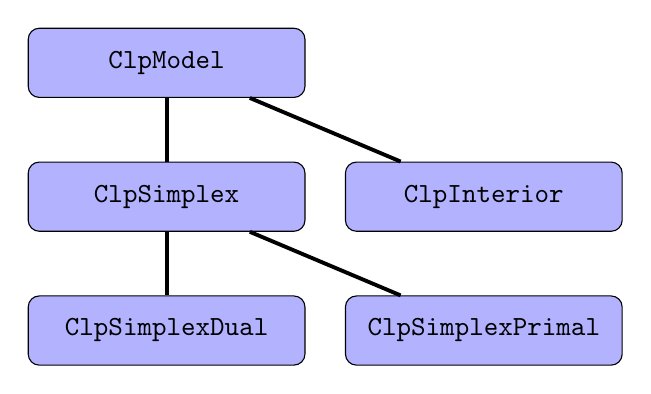
\begin{tikzpicture}[node distance=2.5cm]
    \tikzstyle{every state}=[rectangle,
                             minimum width=10em,
                             rounded corners,
                             fill=blue!30,
                             edge from parent,
                             text=black]
    \tikzset{node distance=1.7cm};

    \node[state] (a)                    {\texttt{ClpModel}};
    \node[state] (b) [below of = a]     {\texttt{ClpSimplex}};
    \node[state] (c) [right = 0.5cm of b] {\texttt{ClpInterior}};
    \node[state] (d) [below of = b]     {\texttt{ClpSimplexDual}};
    \node[state] (e) [right = 0.5cm of d] {\texttt{ClpSimplexPrimal}};

    \tikzset{edgestyle/.style={-, double=black}}
%    \tikzset{every node/.style={fill=white}}

    \path (a) edge [edgestyle] node {}  (b)
          (a) edge [edgestyle] node {}  (c)
          (b) edge [edgestyle] node {}  (d)
          (b) edge [edgestyle] node {}  (e);
\end{tikzpicture}
\caption{Class hierarchy for \texttt{ClpModel}}
\label{fig:clpmodel}
\end{figure}


\section{Slp}
While implementing an algorithm, it makes sense to start to implement
sub-functions that are not dependant on other functions. 

Implementing the Taylor series expansion is pretty straight forward, as
we have a closed-form definition for the specific objective function that
we described in Chapter \ref{ch:qp}. The function prototype for the
Taylor series expansion reads:
\begin{verbatim}
void taylor(double* T, const double* x,
            const ClpModel& m);
\end{verbatim}
where \texttt{ClpModel} gives us access to both the linear and quadratic
objective term. The result of the Taylor-series expansion, i.e. the new
objective function, is put in \texttt{T}.

The next step in the Slp algorithm is to solve the new linear program with the
new objective function \texttt{T}. This is simply done with a call to Clp.

After solving the linear program, the next step is to find the one-dimensional
minimizer between our current point and the solution to the linear program we
just solved.
The step length $\alpha_k$ tells us where this minimizer lies between the two
points.
To implement this line search, we find a closed-form definition of the step
length $\alpha_k$ by letting $m(\alpha) = f((1-\alpha) x_k + \alpha \hat{x}_k)$
and setting $m^\prime(\alpha) = 0$ and solving for $\alpha$:
\[
\alpha_k = \frac{
                2x_k^T H x_k
                - 2\hat{x}_k^T H x_k
                + b^T x_k - b^T \hat{x}_k
                }{
                  2\hat{x}_k^T H \hat{x}_k
                - 4\hat{x}_k^T H x_k
                + 2x_k^T H x_k
                }
\]
The function prototype for the line search function reads:
\begin{verbatim}
double lineSearch(const double* p,
                  const double* q,
                  ClpModel& m);
\end{verbatim}
where \texttt{ClpModel} gives us access to both the linear and quadratic
objective term.

The termination condition of Slp depends on the objective value of the two
previous iterations. So, in order to terminate, we need a function that can
compute the objective value. The function prototype for this function reads:
\begin{verbatim}
double objVal(const double* p, const ClpModel& m);
\end{verbatim}
where \texttt{ClpModel} again gives us access to both the linear and quadratic
objective term.

These three functions all have an asymptotic running time in the order of the
number of columns in the problem, because they do a constant number of
operations while iterating sparsely through matrix $H$ and vector $b$.

When it comes to decisions to be made around data types and storage formats,
there is not really too much to be said, because the choices are quite limited.
It is pretty much dependant on the linear programming solver that is used.
As mentioned earlier, Clp stores matrices in a sparse format, and all the sub
functions only operate on non-zero elements, so there is not really room for
much overhead.

An implementation of Algorithm \ref{alg:iter} in \texttt{C++} looks like this:
\begin{verbatim}
ClpModel lin = m; // A linear copy of ClpModel m
do {
    taylor(T, x, m);

    lin.chgObjCoefficients(T); // Set new linear objective
    lin.primal(); // Run the primal simplex method
    
    const double* xhat = lin.primalColumnSolution(); // Opt. sol
    double alpha = lineSearch(x, xhat, m);
    if      (alpha > 1) alpha = 1;
    else if (alpha < 0) alpha = 0;

    double oldval = objVal(x, m);
    for (int i = 0; i < numCols; i++) {
        x[i] = (1-alpha) * xhat[i];
    }
    double val = objVal(x, m);

    stop = (oldval - val);
    stop /= fabs(oldval);
} while (stop > tolerance);
\end{verbatim}


\section{Solving Subinstances}
In this section, we discuss the implementation of the different approaches to
solving several subinstances.
As mentioned in the beginning of the chapter, the two
main approaches are to solve a limited amount of subinstances, bounded
by $\sigma(\beta, n)$ for some $\beta$ and a problem size $n$, or to implement a discrete
event simulator that only stores the current state of the network.
First we will discuss the implementation of the tree structure, before we
move on to the two main approaches.

\subsection{Tree Structure}
All trees consists of vertices, and in our specific case, each vertex contains
two sets $\mathcal{M}$ and $\mathcal{Z}$, a solution $x^*$, and a number of
child vertices. To keep vertices as simple as possible, we implement them as
simple \texttt{structs}. Each vertex \texttt{struct} looks like
this:
\begin{verbatim}
struct vertex {
  set<uint16_t> m;
  set<uint16_t> z;
  double* sol;
  vector<struct vertex*> children;
};
\end{verbatim}
A reader familiar with \texttt{C++} might notice that we use
\texttt{set} instead of using a bit vector as we discussed
in Section \ref{ch:tree}, and we will come to that later. Note that
the sets consist of indices of primitive type \texttt{uint16\_t}, which is
short for \texttt{unsigned short int}. That means that the sets are limited to
$2^{16} = 65536$ elements, and therefore also putting a limit to the size
of the QP problems that can be solved. This seems like a reasonable limit
as Goodtech wants to solve problems with $200 - 2000$ variables.
If they need to solve larger problems in the future, it is possible to change
the primitive data type.

As soon as a vertex is defined, we are ready to implement \texttt{mfind}.
Remember that \texttt{mfind} is a modified version of \texttt{find} that tells
us which vertex should be the parent of our potentially new vertex in case it
has a distinct solution.
\texttt{mfind} is defined in two parts. The first part is a driver function
for starting the algorithm on some vertex. The second part is the actual
recursively defined algorithm. These two parts are called \texttt{mfind} and
\texttt{mfindrec}, respectively. We define \texttt{mfind} as follows:
\begin{verbatim}
bool mfind(const set<uint16_t>& m,
struct vertex* v, struct vertex*& ret)
{
  ret = v;
  return mfindrec(m, v, ret);
}
\end{verbatim}
The parameters for \texttt{mfind} are a modifier, a vertex where the search
will begin and an output vertex.
In order to search the whole tree, one would use the root vertex as parameter
\texttt{v}.
The function returns a boolean that changes the meaning of the output vertex.
The function makes a call to \texttt{mfindrec}:
\begin{verbatim}
bool mfindrec(const std::set<uint16_t>& m,
struct vertex* v, struct vertex*& ret)
{
  if (isSubset(m, v->z)) return true;
  for (struct vertex* vi : v->children) {
    if (isSubset(vi->m, m)) {
      ret = vi; 
      bool temp = mfindrec(m, vi, ret);
      if (temp) return true;
    }   
  }   
  return false;
}
\end{verbatim}
It is quite evident from the code that the performance of the \texttt{isSubset}
function is important. In Chapter \ref{ch:tree} we discussed using bit vectors 
to represent sets. We concluded that a simple \texttt{AND} operation would tell
us whether a set was a subset of another set.
We also discussed the possibility of it being more memory efficient than
storing sets in a sparse format where only the indices of each variable was
stored.

Using a bit vector, each set consumes exactly $n$ bits of storage if our
\emph{universe} holds $n$ variables.
Using sets of sparsely stored indices, each set consumes a varying amount of
bits depending on how many variables are in the set. If each index is of data
type \texttt{uint16\_t}, then each index consumes $16$ bits. The trade-off
here is quite clear: If a set contains less than one sixteenth of $n$, then
the sparse format uses less memory. This might actually be the case in a lot
of sets, especially when solving all possible subinstances where the number
of breakdowns are limited by some $\beta$. Consider a very small case where
$n = 200$ and we solve all subinstances
$\sigma(3, 200) = \sum_{j=0}^{3} {\binom{200}{j}} = S$.
With a total number of $S$ sets stored as bit vectors, the memory use for
storing the modifiers is $200S~\textrm{bits} \approx 32~\textrm{megabytes}$.
Whereas, with $S$ sets of sparsely stored indices, the memory use for storing
the modifiers is approximately $8$ megabytes. However, as $\beta$ increases,
the greater the benefits of storing sets in bit vectors become evident. As soon
as $\beta$ becomes greater than 12, bit vectors will use less memory to store all
modifiers. Figure \ref{fig:bmem} shows the ratio of memory used by bit vectors
over memory used by sets of sparsely stored indices where $n = 200$ and
$5 \leq \beta \leq 30$.
\begin{figure}[ht!]
\centering
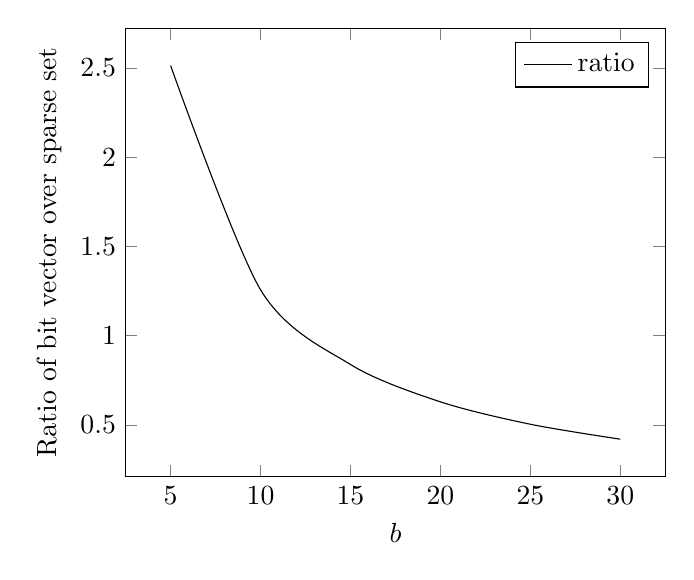
\begin{tikzpicture}
    \begin{axis}[
        legend pos=north east,
        xlabel=$b$,
        ylabel=Ratio of bit vector over sparse set]

        \addplot[black, smooth] plot coordinates {
            (5,  2.51302)
            (10, 1.25686)
            (15, 0.838169)
            (20, 0.628847)
            (25, 0.503276)
            (30, 0.419585)
        };

        \legend{ratio}
    \end{axis}
\end{tikzpicture}

\caption{The ratio of memory use of \texttt{bitset} over \texttt{set} as a
         function of $\beta$.}
\label{fig:bmem}
\end{figure}
Aside from the modifier set, we also have to store the set of variables that
are equal to zero in the optimal solutions of each subinstance. These sets
are more difficult to analyze in terms of memory use, simply because the
cardinality is unknown. However, we do know that $|\mathcal{Z}_k| \geq
|\mathcal{M}_k|$.

With sets of sparsely stored indices, we only need to check the variables
that are actually in the sets in order to determine if a set is a subset
of some set. However, with bit vectors, we need to check $n$ bits---where $n$
is the number of variables in the universe---in order to determine the same.
This means that the \texttt{isSubset} routine will most likely have a different
running time with the two implementations.

One way to find out which of the two are most suited for our need is to perform
a benchmark of the two.
By setting the universe to some size $n$, and generating sets of
random sparsity less than or equal to $n$, we can test how fast
\texttt{isSubset} will run.
We generate random sets as \texttt{bitsets} in \texttt{C++}, storing copies
of these sets in the sparse representation, then testing the performance 
of both implementations of \texttt{isSubset}.
Figure \ref{fig:setspeed}
shows the running time of the two implementations in seconds. Both
implementations were tested on $3000^2$ \texttt{isSubset}-executions, while
increasing $n$.
Codes for the benchmark can be found in Appendix \ref{app:setbench}.
\begin{figure}[ht!]
\centering
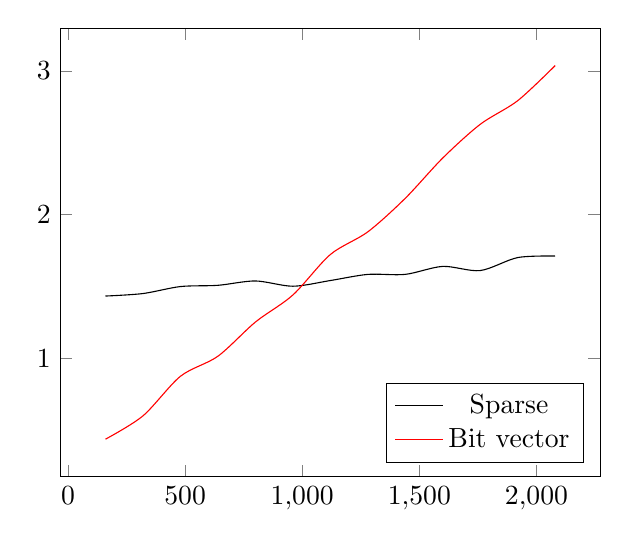
\begin{tikzpicture}
    \begin{axis}[
        legend pos=south east]
%        xlabel=Variables in Universe,
%        ylabel=Seconds]

        \addplot[black, smooth] plot coordinates {
(160, 1.43344)
(320, 1.45082)
(480, 1.49948)
(640, 1.50815)
(800, 1.53846)
(960, 1.50186)
(1120, 1.54138)
(1280, 1.58404)
(1440, 1.58431)
(1600, 1.63973)
(1760, 1.61084)
(1920, 1.70125)
(2080, 1.71173)
        };

        \addplot[red, smooth] plot coordinates {
(160, 0.437256)
(320, 0.599489)
(480, 0.875034)
(640, 1.01462)
(800, 1.25228)
(960, 1.44069)
(1120, 1.72237)
(1280, 1.88017)
(1440, 2.11386)
(1600, 2.39418)
(1760, 2.6287)
(1920, 2.79312)
(2080, 3.03735)
        };

        \legend{Sparse, Bit vector}
    \end{axis}
\end{tikzpicture}

\caption{CPU-seconds used to execute $3000^2$ calls to \texttt{isSubset} on
         randomly generated sets with random sparsity as a function of $n$.}
\label{fig:setspeed}
\end{figure}

We see that the bit vector implementation is much faster than the sparse
implementation on smaller universes. However, the sparse implementation
scales much better than the bit vector implementation when the size of
the universe increases. When it comes to memory, the situation is the same,
except reversed. The sets of sparsely stored indices obviously uses less
memory when $\beta$ is small, i.e. the modifiers are more sparse. However, they
do not scale as nicely as the bit vectors. So the choice relies on what is
most important: memory or speed. Since the nature of this thesis is to
implement a \emph{fast} solver, we give speed a higher priority than memory 
efficiency, so we choose to implement the sets of sparsely stored
indices. That is, in \texttt{C++}, \texttt{set}.

\subsection{Tree Construction}
Because we do not need to store any information about edges in the tree,
we do not need to implement edges as an object of its own. We defined
a vertex \texttt{struct} earlier, having a \texttt{vector} of child
vertices. That means that for each vertex we have, we can reach all child
vertices, children's child vertices and so on, from that vertex.
So, if we have a pointer to the root of a tree, we can reach all vertices
in the tree. Although we earlier defined a tree as an ordered pair
$(V, E)$ of a set of vertices $V$ and a set of edges $E$, we only need a
pointer \texttt{struct vertex*} to our root to access our tree.

The biggest operations in Algorithm \ref{alg:construct} is iterating the power
set of $\left\{1,2,\ldots,n\right\}$. There are lots of combination generators available, so
instead of re-inventing the wheel, we choose a generator that suits our needs.
We need one that is easy to use, and is capable of generating combinations of
a given cardinality. One implementation, similar in use to
\texttt{next\_permutation} in the standard \texttt{C++ STL}, is presented
in~\cite{codeproject}.
Codes from \cite{codeproject} can be found in Appendix
\ref{app:nextcombination}.

The remaining parts of the \texttt{construct}-routine is just running
\texttt{mfind} on each generated modifier, and adding it to the tree
if necessary. Then at the end, return the pointer to the root vertex.

\subsection{Discrete Event Simulation}
In a discrete event simulation (DES), operations are always triggered by events.
In a DES for the reliability analyses discussed in Chapter \ref{ch:intro},
we only need to consider two types of events; a breakdown in the network,
or that a link is repaired.
Each link in the network is represented by
a variable, so each event can by represented by a single variable.

The current state of our system is easily represented by a QP $\mathcal{Q}$ and
a set of variables representing the current broken links in our network.
As this set represents broken links, just like our modifiers $\mathcal{M}_k$
represents breakdowns, we choose to denote the current state of the system
by $\mathcal{M}$. 

Given a variable $x$ to represent a link that breaks down, we need to
update the  current state of the system. This is done with a simple
\textit{union}
\[
\mathcal{M} = \mathcal{M} \cup \left\{x\right\}.
\]
Given a variable $x$ of variables to represent a repaired link, we update the
current state with a simple \textit{relative complement}
\[
\mathcal{M} = \mathcal{M} \setminus \left\{x\right\}.
\]
We call these two operations for \texttt{break} and \texttt{repair}, respectively.
After every change of state in the system, we need to solve the subinstance
of $\mathcal{Q}$ defined by the modifier $\mathcal{M}$.

As the state of the system changes, we need to solve more and more subinstances.
We can choose whether or not we want to store the modifiers and their respective
solutions in a tree or not. If we choose to store distinct solutions in a tree,
we check the tree for a solution for the subinstance defined by the newly
updated modifier, before we potentially solve the problem.


\section{A Quick Overview}
In this section we present a quick overview of the different
implementations.

Although Clp is written primarily for solving linear
programs, it comes with a QP solver. This QP solver uses an implementation
of a primal-dual predictor-corrector interior point method. In addition
to Clp's QP solver, we also have the QP solver presented in Section
\ref{ch:slp}.

There are four different implementations we have, named
\texttt{construct\_clp}, \texttt{construct\_slp}, \texttt{naive\_clp} and
\texttt{naive\_slp}. The implementations with names ending with
\texttt{\_clp} and \texttt{\_slp} uses Clp's QP solver and Slp, respectively,
whenever a QP needs to be solved.
The \texttt{construct} implementations uses the tree structured presented
in Section \ref{ch:tree} for storing subinstances with distinct solutions.
The \texttt{naive} implementations, however, solves subinstances regardless of
whether they have distinct solutions or not.

In the next section, we present several experiments to perform on our
implementations.

\chapter{Implementation}
Recall from Chapter \ref{ch:qp} that we discussed limiting the amount
of subinstances to solve. We did this by introducing a limit on the number of
simultaneous break-downs in the network by some $\beta$.
Another approach is to implement a discrete-event simulator (DES). Each event
occurs at a particular instant in time that changes the state of the system.
In this case, each event would either be a breakdown in the network, or that
a breakdown is fixed.

The difference in these two approaches are prominent, but they share the same
core, namely a QP solver. In this chapter we first discuss the implementation
of the solver declared in Chapter \ref{ch:slp}, before we move on to the
implementation of the two approaches of solving several subinstances.
\label{ch:implementation}

\section{Finding an LP Solver}
The method described in Chapter \ref{ch:slp} relies on repetitively solving
linear programs. Before implementing such a method, it is important to choose
an appropriate LP solver. The solver must
\begin{inparaenum}[\itshape a\upshape)]
\item be released under a free license; and
\item it must allow library calls in C/C++
\end{inparaenum}

Among a list of about 50 solvers (most of them proprietary), the
following three matches the aforementioned criteria:
\begin{description}
\item[Clp] \hfill \\
Clp is short for Coin-or linear programming. It is a free linear programming
solver released under the Common Public License (CPL). It is primarily meant to
be used as a callable library. Its license allows other software to link to the
Clp library without requiring that that software is released under the same
license (permissive). \cite{clp}
\item[GLPK] \hfill \\
GLPK is short for GNU Linear Programming Kit. It is a free linear (integer)
programming software packaged released under the GNU General Public License
(GNU GPL). GLPK is organized in the form of a callable library. Its license
requires linking software to be released under the GNU GPL (reciprocal).
\cite{glpk}
\item[lp\_solve] \hfill \\
lp\_solve is a free linear (integer) programming solver released under the GNU 
Lesser General Public License (GNU LGPL). Its license is permissive like the
CPL. \cite{lpsolve}
\end{description}

Incidentally, these tree solvers are the only three open source LP solvers
suggested by the NEOS Optimization Guide~\cite{neos}.
In addition to the mentioned criteria, it is important that the solver is
fast.
Moreover, it needs to be fast on problems that fit the description in
Section \ref{sec:problem}.

Testing the three solvers on linearized versions of the instances
\textit{small} and \textit{large}---presented in
Chapter \ref{sec:instances}---reveals the running times shown in Table
\ref{table:lpres}.
The running times are the number of seconds in CPU-time after 1000 runs.

\begin{table}[ht!]
    \centering
    \caption{Running time in CPU-seconds used by each solver to solve 1000
             instances of each problem.}
    \begin{tabular}{lrrr}
        Data Set       & Clp    & GLPK   & lp\_solve \\ \hline
        \textit{small} & 6.929  & 26.096 & 4.734 \\
        \textit{large} & 12.832 & 47.977 & 23.376
    \end{tabular}
    \label{table:lpres}
\end{table}

While lp\_solve is the fastest on a smaller LP, it doesn't scale as well as
with larger problems like Clp does.

GoodTech need to solve problems with more than 200 variables, and
\textit{small} is almost hitting that lower limit, so a good result on
\textit{large} is prioritized over the other.
This means that Clp outperforms the other two solvers in this test.

Although this is not an extensive test, it is a pretty good indicator that Clp
will be the fastest solver on similar problems.


\section{Clp}
Clp is written primarily by John J. Forrest, now retired from IBM Research. At
the time of writing, Clp is under active development. It is currently
managed by John Forrest, Julian Hall, Lou Hafer and Matthew Saltzman.
\cite{clppage}

Matrices in Clp are stored in a compact format using three vectors.
The first vector contains all the non-zero elements of the matrix.
The second vector contains the indices of the elements in the first vector.
The third vector contains an accumulated number of elements in each row/column.
The order of the elements depends whether the matrix is row-ordered or
column-ordered.
The indices represent the column/row position of the elements, and the
accumulated values represent the accumulated number of elements in the
row/columns depending on whether the matrix is row-ordered or column-ordered,
respectively.
To get a better understanding of how they are stored, consider the matrix
\[
\left[
\begin{array}{rrrrrrrr}
    3 & 1 & 0   & -2  & -1 & 0 & 0    & -1 \\
    0 & 2 & 1.1 & 0   & 0  & 0 & 0    & 0  \\
    0 & 0 & 1   & 0   & 0  & 1 & 0    & 0  \\
    0 & 0 & 0   & 2.8 & 0  & 0 & -1.2 & 0  \\
  5.6 & 0 & 0   & 0   & 1  & 0 & 0    & 1.9  

\end{array}
\right]
\]
being stored in row-ordered format, then the element vector would be
\[
\begin{array}{l}
\left[
\begin{array}{rrrrrrr}
    3 & 1 & -2 & -1 & -1 & 2 & 1.1
\end{array}\right. \\
\left.\begin{array}{rrrrrrr}
    1 & 1 & 2.8 & -1.2 & 5.6 & 1 & 1.9
\end{array}
\right]^T,
\end{array}
\]
the vector containing the column indices would be
\[
\left[
\begin{array}{rrrrrrrrrrrrrr}
    0 & 1 & 3 & 4 & 7 & 1 & 2 & 2 & 5 & 3 & 6 & 0 & 4 & 7
\end{array}
\right]^T,
\]
and the vector containing the vector starts (the accumulated indices) would be
\[
\left[
\begin{array}{rrrrrr}
    0 & 5 & 7 & 9 & 11 & 14
\end{array}
\right]^T.
\]
The \texttt{CoinPackedMatrix} class represents such a compact matrix.
To keep overhead at a minimum, it is important to implement the new solver
(from here on called Slp) using the same compact format.

Clp has a base class that holds data for both linear and quadratic models
called \texttt{ClpModel}.
The class itself knows nothing about the implementation of the algorithms, but
it contains all the data about a problem needed to apply an algorithm on that
data.
This is very handy for passing data throughout Slp without much overhead.
It also results in very neat function prototypes as only one parameter
is needed for passing lots of information. For instance, the function prototype
in Slp for the function that performs the line search described in Chapter
\ref{ch:slp} looks like this:
\begin{verbatim}
double lineSearch(const double* a,
                  const double* b,
                  ClpModel& m);
\end{verbatim}
Figure \ref{fig:clpmodel} shows the class hierarchy for \texttt{ClpModel}.
The subclasses contain the implementation of the algorithms that their class
names describe. For instance, \texttt{ClpSimplexDual} contains the
implementation of the Dual Simplex Algorithm.
\begin{figure}
\centering
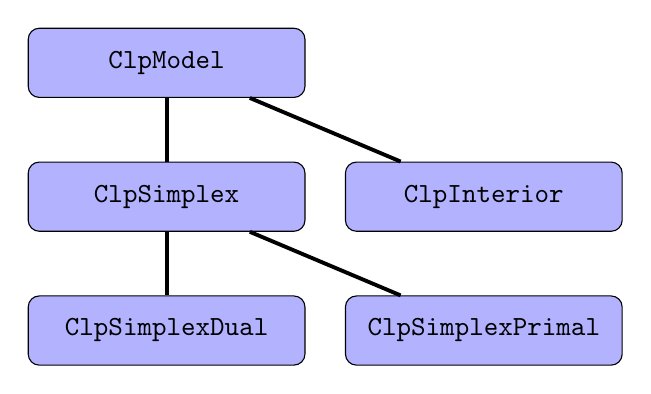
\begin{tikzpicture}[node distance=2.5cm]
    \tikzstyle{every state}=[rectangle,
                             minimum width=10em,
                             rounded corners,
                             fill=blue!30,
                             edge from parent,
                             text=black]
    \tikzset{node distance=1.7cm};

    \node[state] (a)                    {\texttt{ClpModel}};
    \node[state] (b) [below of = a]     {\texttt{ClpSimplex}};
    \node[state] (c) [right = 0.5cm of b] {\texttt{ClpInterior}};
    \node[state] (d) [below of = b]     {\texttt{ClpSimplexDual}};
    \node[state] (e) [right = 0.5cm of d] {\texttt{ClpSimplexPrimal}};

    \tikzset{edgestyle/.style={-, double=black}}
%    \tikzset{every node/.style={fill=white}}

    \path (a) edge [edgestyle] node {}  (b)
          (a) edge [edgestyle] node {}  (c)
          (b) edge [edgestyle] node {}  (d)
          (b) edge [edgestyle] node {}  (e);
\end{tikzpicture}
\caption{Class hierarchy for \texttt{ClpModel}}
\label{fig:clpmodel}
\end{figure}


\section{Slp}
While implementing an algorithm, it makes sense to start to implement
sub-functions that are not dependant on other functions. 

Implementing the Taylor series expansion is pretty straight forward, as
we have a closed-form definition for the specific objective function that
we described in Chapter \ref{ch:qp}. The function prototype for the
Taylor series expansion reads:
\begin{verbatim}
void taylor(double* T, const double* x,
            const ClpModel& m);
\end{verbatim}
where \texttt{ClpModel} gives us access to both the linear and quadratic
objective term. The result of the Taylor-series expansion, i.e. the new
objective function, is put in \texttt{T}.

The next step in the Slp algorithm is to solve the new linear program with the
new objective function \texttt{T}. This is simply done with a call to Clp.

After solving the linear program, the next step is to find the one-dimensional
minimizer between our current point and the solution to the linear program we
just solved.
The step length $\alpha_k$ tells us where this minimizer lies between the two
points.
To implement this line search, we find a closed-form definition of the step
length $\alpha_k$ by letting $m(\alpha) = f((1-\alpha) x_k + \alpha \hat{x}_k)$
and setting $m^\prime(\alpha) = 0$ and solving for $\alpha$:
\[
\alpha_k = \frac{
                2x_k^T H x_k
                - 2\hat{x}_k^T H x_k
                + b^T x_k - b^T \hat{x}_k
                }{
                  2\hat{x}_k^T H \hat{x}_k
                - 4\hat{x}_k^T H x_k
                + 2x_k^T H x_k
                }
\]
The function prototype for the line search function reads:
\begin{verbatim}
double lineSearch(const double* p,
                  const double* q,
                  ClpModel& m);
\end{verbatim}
where \texttt{ClpModel} gives us access to both the linear and quadratic
objective term.

The termination condition of Slp depends on the objective value of the two
previous iterations. So, in order to terminate, we need a function that can
compute the objective value. The function prototype for this function reads:
\begin{verbatim}
double objVal(const double* p, const ClpModel& m);
\end{verbatim}
where \texttt{ClpModel} again gives us access to both the linear and quadratic
objective term.

These three functions all have an asymptotic running time in the order of the
number of columns in the problem, because they do a constant number of
operations while iterating sparsely through matrix $H$ and vector $b$.

When it comes to decisions to be made around data types and storage formats,
there is not really too much to be said, because the choices are quite limited.
It is pretty much dependant on the linear programming solver that is used.
As mentioned earlier, Clp stores matrices in a sparse format, and all the sub
functions only operate on non-zero elements, so there is not really room for
much overhead.

An implementation of Algorithm \ref{alg:iter} in \texttt{C++} looks like this:
\begin{verbatim}
ClpModel lin = m; // A linear copy of ClpModel m
do {
    taylor(T, x, m);

    lin.chgObjCoefficients(T); // Set new linear objective
    lin.primal(); // Run the primal simplex method
    
    const double* xhat = lin.primalColumnSolution(); // Opt. sol
    double alpha = lineSearch(x, xhat, m);
    if      (alpha > 1) alpha = 1;
    else if (alpha < 0) alpha = 0;

    double oldval = objVal(x, m);
    for (int i = 0; i < numCols; i++) {
        x[i] = (1-alpha) * xhat[i];
    }
    double val = objVal(x, m);

    stop = (oldval - val);
    stop /= fabs(oldval);
} while (stop > tolerance);
\end{verbatim}


\section{Solving Subinstances}
In this section, we discuss the implementation of the different approaches to
solving several subinstances.
As mentioned in the beginning of the chapter, the two
main approaches are to solve a limited amount of subinstances, bounded
by $\sigma(\beta, n)$ for some $\beta$ and a problem size $n$, or to implement a discrete
event simulator that only stores the current state of the network.
First we will discuss the implementation of the tree structure, before we
move on to the two main approaches.

\subsection{Tree Structure}
All trees consists of vertices, and in our specific case, each vertex contains
two sets $\mathcal{M}$ and $\mathcal{Z}$, a solution $x^*$, and a number of
child vertices. To keep vertices as simple as possible, we implement them as
simple \texttt{structs}. Each vertex \texttt{struct} looks like
this:
\begin{verbatim}
struct vertex {
  set<uint16_t> m;
  set<uint16_t> z;
  double* sol;
  vector<struct vertex*> children;
};
\end{verbatim}
A reader familiar with \texttt{C++} might notice that we use
\texttt{set} instead of using a bit vector as we discussed
in Section \ref{ch:tree}, and we will come to that later. Note that
the sets consist of indices of primitive type \texttt{uint16\_t}, which is
short for \texttt{unsigned short int}. That means that the sets are limited to
$2^{16} = 65536$ elements, and therefore also putting a limit to the size
of the QP problems that can be solved. This seems like a reasonable limit
as Goodtech wants to solve problems with $200 - 2000$ variables.
If they need to solve larger problems in the future, it is possible to change
the primitive data type.

As soon as a vertex is defined, we are ready to implement \texttt{mfind}.
Remember that \texttt{mfind} is a modified version of \texttt{find} that tells
us which vertex should be the parent of our potentially new vertex in case it
has a distinct solution.
\texttt{mfind} is defined in two parts. The first part is a driver function
for starting the algorithm on some vertex. The second part is the actual
recursively defined algorithm. These two parts are called \texttt{mfind} and
\texttt{mfindrec}, respectively. We define \texttt{mfind} as follows:
\begin{verbatim}
bool mfind(const set<uint16_t>& m,
struct vertex* v, struct vertex*& ret)
{
  ret = v;
  return mfindrec(m, v, ret);
}
\end{verbatim}
The parameters for \texttt{mfind} are a modifier, a vertex where the search
will begin and an output vertex.
In order to search the whole tree, one would use the root vertex as parameter
\texttt{v}.
The function returns a boolean that changes the meaning of the output vertex.
The function makes a call to \texttt{mfindrec}:
\begin{verbatim}
bool mfindrec(const std::set<uint16_t>& m,
struct vertex* v, struct vertex*& ret)
{
  if (isSubset(m, v->z)) return true;
  for (struct vertex* vi : v->children) {
    if (isSubset(vi->m, m)) {
      ret = vi; 
      bool temp = mfindrec(m, vi, ret);
      if (temp) return true;
    }   
  }   
  return false;
}
\end{verbatim}
It is quite evident from the code that the performance of the \texttt{isSubset}
function is important. In Chapter \ref{ch:tree} we discussed using bit vectors 
to represent sets. We concluded that a simple \texttt{AND} operation would tell
us whether a set was a subset of another set.
We also discussed the possibility of it being more memory efficient than
storing sets in a sparse format where only the indices of each variable was
stored.

Using a bit vector, each set consumes exactly $n$ bits of storage if our
\emph{universe} holds $n$ variables.
Using sets of sparsely stored indices, each set consumes a varying amount of
bits depending on how many variables are in the set. If each index is of data
type \texttt{uint16\_t}, then each index consumes $16$ bits. The trade-off
here is quite clear: If a set contains less than one sixteenth of $n$, then
the sparse format uses less memory. This might actually be the case in a lot
of sets, especially when solving all possible subinstances where the number
of breakdowns are limited by some $\beta$. Consider a very small case where
$n = 200$ and we solve all subinstances
$\sigma(3, 200) = \sum_{j=0}^{3} {\binom{200}{j}} = S$.
With a total number of $S$ sets stored as bit vectors, the memory use for
storing the modifiers is $200S~\textrm{bits} \approx 32~\textrm{megabytes}$.
Whereas, with $S$ sets of sparsely stored indices, the memory use for storing
the modifiers is approximately $8$ megabytes. However, as $\beta$ increases,
the greater the benefits of storing sets in bit vectors become evident. As soon
as $\beta$ becomes greater than 12, bit vectors will use less memory to store all
modifiers. Figure \ref{fig:bmem} shows the ratio of memory used by bit vectors
over memory used by sets of sparsely stored indices where $n = 200$ and
$5 \leq \beta \leq 30$.
\begin{figure}[ht!]
\centering
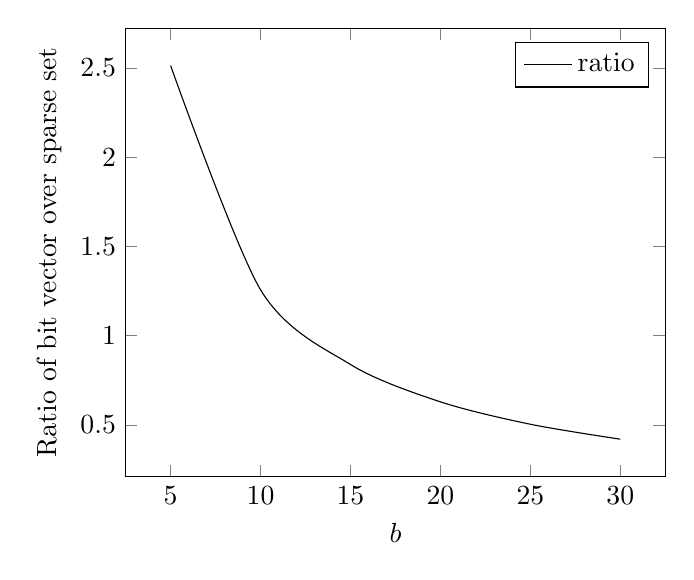
\begin{tikzpicture}
    \begin{axis}[
        legend pos=north east,
        xlabel=$b$,
        ylabel=Ratio of bit vector over sparse set]

        \addplot[black, smooth] plot coordinates {
            (5,  2.51302)
            (10, 1.25686)
            (15, 0.838169)
            (20, 0.628847)
            (25, 0.503276)
            (30, 0.419585)
        };

        \legend{ratio}
    \end{axis}
\end{tikzpicture}

\caption{The ratio of memory use of \texttt{bitset} over \texttt{set} as a
         function of $\beta$.}
\label{fig:bmem}
\end{figure}
Aside from the modifier set, we also have to store the set of variables that
are equal to zero in the optimal solutions of each subinstance. These sets
are more difficult to analyze in terms of memory use, simply because the
cardinality is unknown. However, we do know that $|\mathcal{Z}_k| \geq
|\mathcal{M}_k|$.

With sets of sparsely stored indices, we only need to check the variables
that are actually in the sets in order to determine if a set is a subset
of some set. However, with bit vectors, we need to check $n$ bits---where $n$
is the number of variables in the universe---in order to determine the same.
This means that the \texttt{isSubset} routine will most likely have a different
running time with the two implementations.

One way to find out which of the two are most suited for our need is to perform
a benchmark of the two.
By setting the universe to some size $n$, and generating sets of
random sparsity less than or equal to $n$, we can test how fast
\texttt{isSubset} will run.
We generate random sets as \texttt{bitsets} in \texttt{C++}, storing copies
of these sets in the sparse representation, then testing the performance 
of both implementations of \texttt{isSubset}.
Figure \ref{fig:setspeed}
shows the running time of the two implementations in seconds. Both
implementations were tested on $3000^2$ \texttt{isSubset}-executions, while
increasing $n$.
Codes for the benchmark can be found in Appendix \ref{app:setbench}.
\begin{figure}[ht!]
\centering
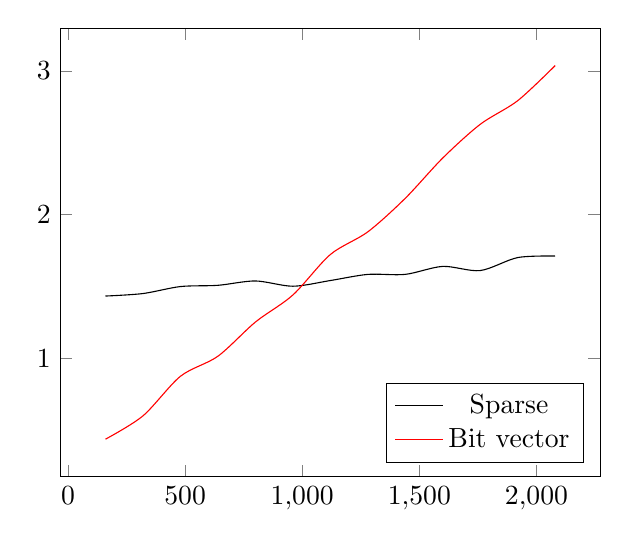
\begin{tikzpicture}
    \begin{axis}[
        legend pos=south east]
%        xlabel=Variables in Universe,
%        ylabel=Seconds]

        \addplot[black, smooth] plot coordinates {
(160, 1.43344)
(320, 1.45082)
(480, 1.49948)
(640, 1.50815)
(800, 1.53846)
(960, 1.50186)
(1120, 1.54138)
(1280, 1.58404)
(1440, 1.58431)
(1600, 1.63973)
(1760, 1.61084)
(1920, 1.70125)
(2080, 1.71173)
        };

        \addplot[red, smooth] plot coordinates {
(160, 0.437256)
(320, 0.599489)
(480, 0.875034)
(640, 1.01462)
(800, 1.25228)
(960, 1.44069)
(1120, 1.72237)
(1280, 1.88017)
(1440, 2.11386)
(1600, 2.39418)
(1760, 2.6287)
(1920, 2.79312)
(2080, 3.03735)
        };

        \legend{Sparse, Bit vector}
    \end{axis}
\end{tikzpicture}

\caption{CPU-seconds used to execute $3000^2$ calls to \texttt{isSubset} on
         randomly generated sets with random sparsity as a function of $n$.}
\label{fig:setspeed}
\end{figure}

We see that the bit vector implementation is much faster than the sparse
implementation on smaller universes. However, the sparse implementation
scales much better than the bit vector implementation when the size of
the universe increases. When it comes to memory, the situation is the same,
except reversed. The sets of sparsely stored indices obviously uses less
memory when $\beta$ is small, i.e. the modifiers are more sparse. However, they
do not scale as nicely as the bit vectors. So the choice relies on what is
most important: memory or speed. Since the nature of this thesis is to
implement a \emph{fast} solver, we give speed a higher priority than memory 
efficiency, so we choose to implement the sets of sparsely stored
indices. That is, in \texttt{C++}, \texttt{set}.

\subsection{Tree Construction}
Because we do not need to store any information about edges in the tree,
we do not need to implement edges as an object of its own. We defined
a vertex \texttt{struct} earlier, having a \texttt{vector} of child
vertices. That means that for each vertex we have, we can reach all child
vertices, children's child vertices and so on, from that vertex.
So, if we have a pointer to the root of a tree, we can reach all vertices
in the tree. Although we earlier defined a tree as an ordered pair
$(V, E)$ of a set of vertices $V$ and a set of edges $E$, we only need a
pointer \texttt{struct vertex*} to our root to access our tree.

The biggest operations in Algorithm \ref{alg:construct} is iterating the power
set of $\left\{1,2,\ldots,n\right\}$. There are lots of combination generators available, so
instead of re-inventing the wheel, we choose a generator that suits our needs.
We need one that is easy to use, and is capable of generating combinations of
a given cardinality. One implementation, similar in use to
\texttt{next\_permutation} in the standard \texttt{C++ STL}, is presented
in~\cite{codeproject}.
Codes from \cite{codeproject} can be found in Appendix
\ref{app:nextcombination}.

The remaining parts of the \texttt{construct}-routine is just running
\texttt{mfind} on each generated modifier, and adding it to the tree
if necessary. Then at the end, return the pointer to the root vertex.

\subsection{Discrete Event Simulation}
In a discrete event simulation (DES), operations are always triggered by events.
In a DES for the reliability analyses discussed in Chapter \ref{ch:intro},
we only need to consider two types of events; a breakdown in the network,
or that a link is repaired.
Each link in the network is represented by
a variable, so each event can by represented by a single variable.

The current state of our system is easily represented by a QP $\mathcal{Q}$ and
a set of variables representing the current broken links in our network.
As this set represents broken links, just like our modifiers $\mathcal{M}_k$
represents breakdowns, we choose to denote the current state of the system
by $\mathcal{M}$. 

Given a variable $x$ to represent a link that breaks down, we need to
update the  current state of the system. This is done with a simple
\textit{union}
\[
\mathcal{M} = \mathcal{M} \cup \left\{x\right\}.
\]
Given a variable $x$ of variables to represent a repaired link, we update the
current state with a simple \textit{relative complement}
\[
\mathcal{M} = \mathcal{M} \setminus \left\{x\right\}.
\]
We call these two operations for \texttt{break} and \texttt{repair}, respectively.
After every change of state in the system, we need to solve the subinstance
of $\mathcal{Q}$ defined by the modifier $\mathcal{M}$.

As the state of the system changes, we need to solve more and more subinstances.
We can choose whether or not we want to store the modifiers and their respective
solutions in a tree or not. If we choose to store distinct solutions in a tree,
we check the tree for a solution for the subinstance defined by the newly
updated modifier, before we potentially solve the problem.


\section{A Quick Overview}
In this section we present a quick overview of the different
implementations.

Although Clp is written primarily for solving linear
programs, it comes with a QP solver. This QP solver uses an implementation
of a primal-dual predictor-corrector interior point method. In addition
to Clp's QP solver, we also have the QP solver presented in Section
\ref{ch:slp}.

There are four different implementations we have, named
\texttt{construct\_clp}, \texttt{construct\_slp}, \texttt{naive\_clp} and
\texttt{naive\_slp}. The implementations with names ending with
\texttt{\_clp} and \texttt{\_slp} uses Clp's QP solver and Slp, respectively,
whenever a QP needs to be solved.
The \texttt{construct} implementations uses the tree structured presented
in Section \ref{ch:tree} for storing subinstances with distinct solutions.
The \texttt{naive} implementations, however, solves subinstances regardless of
whether they have distinct solutions or not.

In the next section, we present several experiments to perform on our
implementations.

\chapter{Implementation}
Recall from Chapter \ref{ch:qp} that we discussed limiting the amount
of subinstances to solve. We did this by introducing a limit on the number of
simultaneous break-downs in the network by some $\beta$.
Another approach is to implement a discrete-event simulator (DES). Each event
occurs at a particular instant in time that changes the state of the system.
In this case, each event would either be a breakdown in the network, or that
a breakdown is fixed.

The difference in these two approaches are prominent, but they share the same
core, namely a QP solver. In this chapter we first discuss the implementation
of the solver declared in Chapter \ref{ch:slp}, before we move on to the
implementation of the two approaches of solving several subinstances.
\label{ch:implementation}

\section{Finding an LP Solver}
The method described in Chapter \ref{ch:slp} relies on repetitively solving
linear programs. Before implementing such a method, it is important to choose
an appropriate LP solver. The solver must
\begin{inparaenum}[\itshape a\upshape)]
\item be released under a free license; and
\item it must allow library calls in C/C++
\end{inparaenum}

Among a list of about 50 solvers (most of them proprietary), the
following three matches the aforementioned criteria:
\begin{description}
\item[Clp] \hfill \\
Clp is short for Coin-or linear programming. It is a free linear programming
solver released under the Common Public License (CPL). It is primarily meant to
be used as a callable library. Its license allows other software to link to the
Clp library without requiring that that software is released under the same
license (permissive). \cite{clp}
\item[GLPK] \hfill \\
GLPK is short for GNU Linear Programming Kit. It is a free linear (integer)
programming software packaged released under the GNU General Public License
(GNU GPL). GLPK is organized in the form of a callable library. Its license
requires linking software to be released under the GNU GPL (reciprocal).
\cite{glpk}
\item[lp\_solve] \hfill \\
lp\_solve is a free linear (integer) programming solver released under the GNU 
Lesser General Public License (GNU LGPL). Its license is permissive like the
CPL. \cite{lpsolve}
\end{description}

Incidentally, these tree solvers are the only three open source LP solvers
suggested by the NEOS Optimization Guide~\cite{neos}.
In addition to the mentioned criteria, it is important that the solver is
fast.
Moreover, it needs to be fast on problems that fit the description in
Section \ref{sec:problem}.

Testing the three solvers on linearized versions of the instances
\textit{small} and \textit{large}---presented in
Chapter \ref{sec:instances}---reveals the running times shown in Table
\ref{table:lpres}.
The running times are the number of seconds in CPU-time after 1000 runs.

\begin{table}[ht!]
    \centering
    \caption{Running time in CPU-seconds used by each solver to solve 1000
             instances of each problem.}
    \begin{tabular}{lrrr}
        Data Set       & Clp    & GLPK   & lp\_solve \\ \hline
        \textit{small} & 6.929  & 26.096 & 4.734 \\
        \textit{large} & 12.832 & 47.977 & 23.376
    \end{tabular}
    \label{table:lpres}
\end{table}

While lp\_solve is the fastest on a smaller LP, it doesn't scale as well as
with larger problems like Clp does.

GoodTech need to solve problems with more than 200 variables, and
\textit{small} is almost hitting that lower limit, so a good result on
\textit{large} is prioritized over the other.
This means that Clp outperforms the other two solvers in this test.

Although this is not an extensive test, it is a pretty good indicator that Clp
will be the fastest solver on similar problems.


\section{Clp}
Clp is written primarily by John J. Forrest, now retired from IBM Research. At
the time of writing, Clp is under active development. It is currently
managed by John Forrest, Julian Hall, Lou Hafer and Matthew Saltzman.
\cite{clppage}

Matrices in Clp are stored in a compact format using three vectors.
The first vector contains all the non-zero elements of the matrix.
The second vector contains the indices of the elements in the first vector.
The third vector contains an accumulated number of elements in each row/column.
The order of the elements depends whether the matrix is row-ordered or
column-ordered.
The indices represent the column/row position of the elements, and the
accumulated values represent the accumulated number of elements in the
row/columns depending on whether the matrix is row-ordered or column-ordered,
respectively.
To get a better understanding of how they are stored, consider the matrix
\[
\left[
\begin{array}{rrrrrrrr}
    3 & 1 & 0   & -2  & -1 & 0 & 0    & -1 \\
    0 & 2 & 1.1 & 0   & 0  & 0 & 0    & 0  \\
    0 & 0 & 1   & 0   & 0  & 1 & 0    & 0  \\
    0 & 0 & 0   & 2.8 & 0  & 0 & -1.2 & 0  \\
  5.6 & 0 & 0   & 0   & 1  & 0 & 0    & 1.9  

\end{array}
\right]
\]
being stored in row-ordered format, then the element vector would be
\[
\begin{array}{l}
\left[
\begin{array}{rrrrrrr}
    3 & 1 & -2 & -1 & -1 & 2 & 1.1
\end{array}\right. \\
\left.\begin{array}{rrrrrrr}
    1 & 1 & 2.8 & -1.2 & 5.6 & 1 & 1.9
\end{array}
\right]^T,
\end{array}
\]
the vector containing the column indices would be
\[
\left[
\begin{array}{rrrrrrrrrrrrrr}
    0 & 1 & 3 & 4 & 7 & 1 & 2 & 2 & 5 & 3 & 6 & 0 & 4 & 7
\end{array}
\right]^T,
\]
and the vector containing the vector starts (the accumulated indices) would be
\[
\left[
\begin{array}{rrrrrr}
    0 & 5 & 7 & 9 & 11 & 14
\end{array}
\right]^T.
\]
The \texttt{CoinPackedMatrix} class represents such a compact matrix.
To keep overhead at a minimum, it is important to implement the new solver
(from here on called Slp) using the same compact format.

Clp has a base class that holds data for both linear and quadratic models
called \texttt{ClpModel}.
The class itself knows nothing about the implementation of the algorithms, but
it contains all the data about a problem needed to apply an algorithm on that
data.
This is very handy for passing data throughout Slp without much overhead.
It also results in very neat function prototypes as only one parameter
is needed for passing lots of information. For instance, the function prototype
in Slp for the function that performs the line search described in Chapter
\ref{ch:slp} looks like this:
\begin{verbatim}
double lineSearch(const double* a,
                  const double* b,
                  ClpModel& m);
\end{verbatim}
Figure \ref{fig:clpmodel} shows the class hierarchy for \texttt{ClpModel}.
The subclasses contain the implementation of the algorithms that their class
names describe. For instance, \texttt{ClpSimplexDual} contains the
implementation of the Dual Simplex Algorithm.
\begin{figure}
\centering
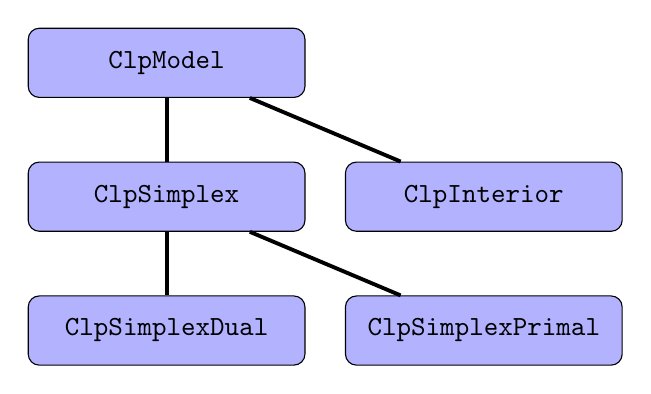
\begin{tikzpicture}[node distance=2.5cm]
    \tikzstyle{every state}=[rectangle,
                             minimum width=10em,
                             rounded corners,
                             fill=blue!30,
                             edge from parent,
                             text=black]
    \tikzset{node distance=1.7cm};

    \node[state] (a)                    {\texttt{ClpModel}};
    \node[state] (b) [below of = a]     {\texttt{ClpSimplex}};
    \node[state] (c) [right = 0.5cm of b] {\texttt{ClpInterior}};
    \node[state] (d) [below of = b]     {\texttt{ClpSimplexDual}};
    \node[state] (e) [right = 0.5cm of d] {\texttt{ClpSimplexPrimal}};

    \tikzset{edgestyle/.style={-, double=black}}
%    \tikzset{every node/.style={fill=white}}

    \path (a) edge [edgestyle] node {}  (b)
          (a) edge [edgestyle] node {}  (c)
          (b) edge [edgestyle] node {}  (d)
          (b) edge [edgestyle] node {}  (e);
\end{tikzpicture}
\caption{Class hierarchy for \texttt{ClpModel}}
\label{fig:clpmodel}
\end{figure}


\section{Slp}
While implementing an algorithm, it makes sense to start to implement
sub-functions that are not dependant on other functions. 

Implementing the Taylor series expansion is pretty straight forward, as
we have a closed-form definition for the specific objective function that
we described in Chapter \ref{ch:qp}. The function prototype for the
Taylor series expansion reads:
\begin{verbatim}
void taylor(double* T, const double* x,
            const ClpModel& m);
\end{verbatim}
where \texttt{ClpModel} gives us access to both the linear and quadratic
objective term. The result of the Taylor-series expansion, i.e. the new
objective function, is put in \texttt{T}.

The next step in the Slp algorithm is to solve the new linear program with the
new objective function \texttt{T}. This is simply done with a call to Clp.

After solving the linear program, the next step is to find the one-dimensional
minimizer between our current point and the solution to the linear program we
just solved.
The step length $\alpha_k$ tells us where this minimizer lies between the two
points.
To implement this line search, we find a closed-form definition of the step
length $\alpha_k$ by letting $m(\alpha) = f((1-\alpha) x_k + \alpha \hat{x}_k)$
and setting $m^\prime(\alpha) = 0$ and solving for $\alpha$:
\[
\alpha_k = \frac{
                2x_k^T H x_k
                - 2\hat{x}_k^T H x_k
                + b^T x_k - b^T \hat{x}_k
                }{
                  2\hat{x}_k^T H \hat{x}_k
                - 4\hat{x}_k^T H x_k
                + 2x_k^T H x_k
                }
\]
The function prototype for the line search function reads:
\begin{verbatim}
double lineSearch(const double* p,
                  const double* q,
                  ClpModel& m);
\end{verbatim}
where \texttt{ClpModel} gives us access to both the linear and quadratic
objective term.

The termination condition of Slp depends on the objective value of the two
previous iterations. So, in order to terminate, we need a function that can
compute the objective value. The function prototype for this function reads:
\begin{verbatim}
double objVal(const double* p, const ClpModel& m);
\end{verbatim}
where \texttt{ClpModel} again gives us access to both the linear and quadratic
objective term.

These three functions all have an asymptotic running time in the order of the
number of columns in the problem, because they do a constant number of
operations while iterating sparsely through matrix $H$ and vector $b$.

When it comes to decisions to be made around data types and storage formats,
there is not really too much to be said, because the choices are quite limited.
It is pretty much dependant on the linear programming solver that is used.
As mentioned earlier, Clp stores matrices in a sparse format, and all the sub
functions only operate on non-zero elements, so there is not really room for
much overhead.

An implementation of Algorithm \ref{alg:iter} in \texttt{C++} looks like this:
\begin{verbatim}
ClpModel lin = m; // A linear copy of ClpModel m
do {
    taylor(T, x, m);

    lin.chgObjCoefficients(T); // Set new linear objective
    lin.primal(); // Run the primal simplex method
    
    const double* xhat = lin.primalColumnSolution(); // Opt. sol
    double alpha = lineSearch(x, xhat, m);
    if      (alpha > 1) alpha = 1;
    else if (alpha < 0) alpha = 0;

    double oldval = objVal(x, m);
    for (int i = 0; i < numCols; i++) {
        x[i] = (1-alpha) * xhat[i];
    }
    double val = objVal(x, m);

    stop = (oldval - val);
    stop /= fabs(oldval);
} while (stop > tolerance);
\end{verbatim}


\section{Solving Subinstances}
In this section, we discuss the implementation of the different approaches to
solving several subinstances.
As mentioned in the beginning of the chapter, the two
main approaches are to solve a limited amount of subinstances, bounded
by $\sigma(\beta, n)$ for some $\beta$ and a problem size $n$, or to implement a discrete
event simulator that only stores the current state of the network.
First we will discuss the implementation of the tree structure, before we
move on to the two main approaches.

\subsection{Tree Structure}
All trees consists of vertices, and in our specific case, each vertex contains
two sets $\mathcal{M}$ and $\mathcal{Z}$, a solution $x^*$, and a number of
child vertices. To keep vertices as simple as possible, we implement them as
simple \texttt{structs}. Each vertex \texttt{struct} looks like
this:
\begin{verbatim}
struct vertex {
  set<uint16_t> m;
  set<uint16_t> z;
  double* sol;
  vector<struct vertex*> children;
};
\end{verbatim}
A reader familiar with \texttt{C++} might notice that we use
\texttt{set} instead of using a bit vector as we discussed
in Section \ref{ch:tree}, and we will come to that later. Note that
the sets consist of indices of primitive type \texttt{uint16\_t}, which is
short for \texttt{unsigned short int}. That means that the sets are limited to
$2^{16} = 65536$ elements, and therefore also putting a limit to the size
of the QP problems that can be solved. This seems like a reasonable limit
as Goodtech wants to solve problems with $200 - 2000$ variables.
If they need to solve larger problems in the future, it is possible to change
the primitive data type.

As soon as a vertex is defined, we are ready to implement \texttt{mfind}.
Remember that \texttt{mfind} is a modified version of \texttt{find} that tells
us which vertex should be the parent of our potentially new vertex in case it
has a distinct solution.
\texttt{mfind} is defined in two parts. The first part is a driver function
for starting the algorithm on some vertex. The second part is the actual
recursively defined algorithm. These two parts are called \texttt{mfind} and
\texttt{mfindrec}, respectively. We define \texttt{mfind} as follows:
\begin{verbatim}
bool mfind(const set<uint16_t>& m,
struct vertex* v, struct vertex*& ret)
{
  ret = v;
  return mfindrec(m, v, ret);
}
\end{verbatim}
The parameters for \texttt{mfind} are a modifier, a vertex where the search
will begin and an output vertex.
In order to search the whole tree, one would use the root vertex as parameter
\texttt{v}.
The function returns a boolean that changes the meaning of the output vertex.
The function makes a call to \texttt{mfindrec}:
\begin{verbatim}
bool mfindrec(const std::set<uint16_t>& m,
struct vertex* v, struct vertex*& ret)
{
  if (isSubset(m, v->z)) return true;
  for (struct vertex* vi : v->children) {
    if (isSubset(vi->m, m)) {
      ret = vi; 
      bool temp = mfindrec(m, vi, ret);
      if (temp) return true;
    }   
  }   
  return false;
}
\end{verbatim}
It is quite evident from the code that the performance of the \texttt{isSubset}
function is important. In Chapter \ref{ch:tree} we discussed using bit vectors 
to represent sets. We concluded that a simple \texttt{AND} operation would tell
us whether a set was a subset of another set.
We also discussed the possibility of it being more memory efficient than
storing sets in a sparse format where only the indices of each variable was
stored.

Using a bit vector, each set consumes exactly $n$ bits of storage if our
\emph{universe} holds $n$ variables.
Using sets of sparsely stored indices, each set consumes a varying amount of
bits depending on how many variables are in the set. If each index is of data
type \texttt{uint16\_t}, then each index consumes $16$ bits. The trade-off
here is quite clear: If a set contains less than one sixteenth of $n$, then
the sparse format uses less memory. This might actually be the case in a lot
of sets, especially when solving all possible subinstances where the number
of breakdowns are limited by some $\beta$. Consider a very small case where
$n = 200$ and we solve all subinstances
$\sigma(3, 200) = \sum_{j=0}^{3} {\binom{200}{j}} = S$.
With a total number of $S$ sets stored as bit vectors, the memory use for
storing the modifiers is $200S~\textrm{bits} \approx 32~\textrm{megabytes}$.
Whereas, with $S$ sets of sparsely stored indices, the memory use for storing
the modifiers is approximately $8$ megabytes. However, as $\beta$ increases,
the greater the benefits of storing sets in bit vectors become evident. As soon
as $\beta$ becomes greater than 12, bit vectors will use less memory to store all
modifiers. Figure \ref{fig:bmem} shows the ratio of memory used by bit vectors
over memory used by sets of sparsely stored indices where $n = 200$ and
$5 \leq \beta \leq 30$.
\begin{figure}[ht!]
\centering
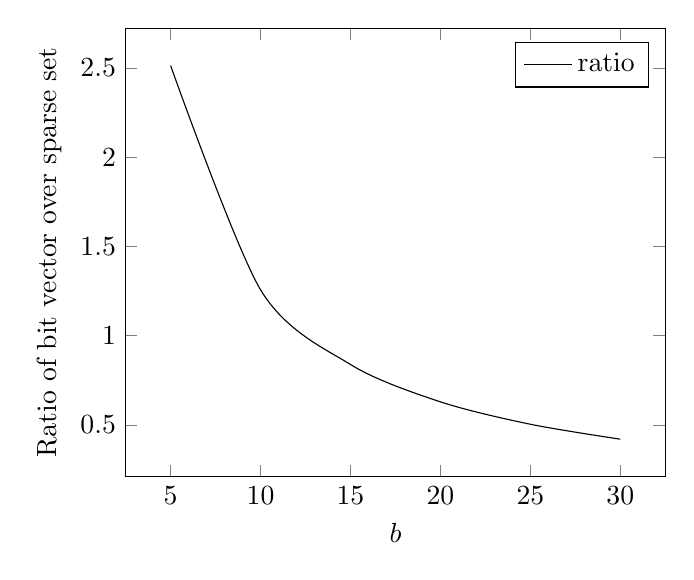
\begin{tikzpicture}
    \begin{axis}[
        legend pos=north east,
        xlabel=$b$,
        ylabel=Ratio of bit vector over sparse set]

        \addplot[black, smooth] plot coordinates {
            (5,  2.51302)
            (10, 1.25686)
            (15, 0.838169)
            (20, 0.628847)
            (25, 0.503276)
            (30, 0.419585)
        };

        \legend{ratio}
    \end{axis}
\end{tikzpicture}

\caption{The ratio of memory use of \texttt{bitset} over \texttt{set} as a
         function of $\beta$.}
\label{fig:bmem}
\end{figure}
Aside from the modifier set, we also have to store the set of variables that
are equal to zero in the optimal solutions of each subinstance. These sets
are more difficult to analyze in terms of memory use, simply because the
cardinality is unknown. However, we do know that $|\mathcal{Z}_k| \geq
|\mathcal{M}_k|$.

With sets of sparsely stored indices, we only need to check the variables
that are actually in the sets in order to determine if a set is a subset
of some set. However, with bit vectors, we need to check $n$ bits---where $n$
is the number of variables in the universe---in order to determine the same.
This means that the \texttt{isSubset} routine will most likely have a different
running time with the two implementations.

One way to find out which of the two are most suited for our need is to perform
a benchmark of the two.
By setting the universe to some size $n$, and generating sets of
random sparsity less than or equal to $n$, we can test how fast
\texttt{isSubset} will run.
We generate random sets as \texttt{bitsets} in \texttt{C++}, storing copies
of these sets in the sparse representation, then testing the performance 
of both implementations of \texttt{isSubset}.
Figure \ref{fig:setspeed}
shows the running time of the two implementations in seconds. Both
implementations were tested on $3000^2$ \texttt{isSubset}-executions, while
increasing $n$.
Codes for the benchmark can be found in Appendix \ref{app:setbench}.
\begin{figure}[ht!]
\centering
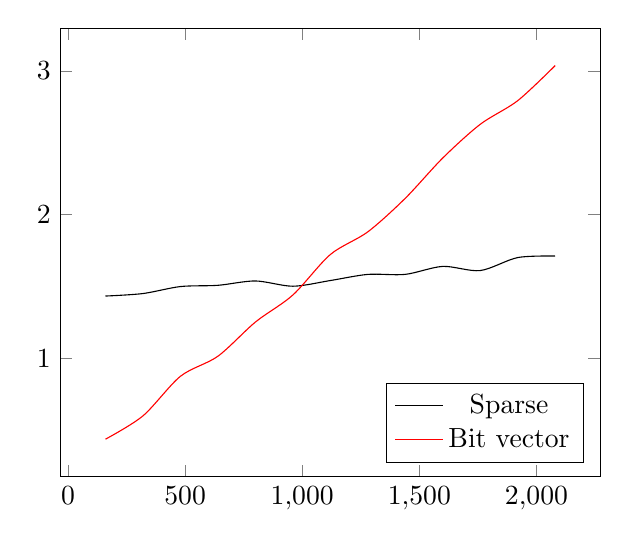
\begin{tikzpicture}
    \begin{axis}[
        legend pos=south east]
%        xlabel=Variables in Universe,
%        ylabel=Seconds]

        \addplot[black, smooth] plot coordinates {
(160, 1.43344)
(320, 1.45082)
(480, 1.49948)
(640, 1.50815)
(800, 1.53846)
(960, 1.50186)
(1120, 1.54138)
(1280, 1.58404)
(1440, 1.58431)
(1600, 1.63973)
(1760, 1.61084)
(1920, 1.70125)
(2080, 1.71173)
        };

        \addplot[red, smooth] plot coordinates {
(160, 0.437256)
(320, 0.599489)
(480, 0.875034)
(640, 1.01462)
(800, 1.25228)
(960, 1.44069)
(1120, 1.72237)
(1280, 1.88017)
(1440, 2.11386)
(1600, 2.39418)
(1760, 2.6287)
(1920, 2.79312)
(2080, 3.03735)
        };

        \legend{Sparse, Bit vector}
    \end{axis}
\end{tikzpicture}

\caption{CPU-seconds used to execute $3000^2$ calls to \texttt{isSubset} on
         randomly generated sets with random sparsity as a function of $n$.}
\label{fig:setspeed}
\end{figure}

We see that the bit vector implementation is much faster than the sparse
implementation on smaller universes. However, the sparse implementation
scales much better than the bit vector implementation when the size of
the universe increases. When it comes to memory, the situation is the same,
except reversed. The sets of sparsely stored indices obviously uses less
memory when $\beta$ is small, i.e. the modifiers are more sparse. However, they
do not scale as nicely as the bit vectors. So the choice relies on what is
most important: memory or speed. Since the nature of this thesis is to
implement a \emph{fast} solver, we give speed a higher priority than memory 
efficiency, so we choose to implement the sets of sparsely stored
indices. That is, in \texttt{C++}, \texttt{set}.

\subsection{Tree Construction}
Because we do not need to store any information about edges in the tree,
we do not need to implement edges as an object of its own. We defined
a vertex \texttt{struct} earlier, having a \texttt{vector} of child
vertices. That means that for each vertex we have, we can reach all child
vertices, children's child vertices and so on, from that vertex.
So, if we have a pointer to the root of a tree, we can reach all vertices
in the tree. Although we earlier defined a tree as an ordered pair
$(V, E)$ of a set of vertices $V$ and a set of edges $E$, we only need a
pointer \texttt{struct vertex*} to our root to access our tree.

The biggest operations in Algorithm \ref{alg:construct} is iterating the power
set of $\left\{1,2,\ldots,n\right\}$. There are lots of combination generators available, so
instead of re-inventing the wheel, we choose a generator that suits our needs.
We need one that is easy to use, and is capable of generating combinations of
a given cardinality. One implementation, similar in use to
\texttt{next\_permutation} in the standard \texttt{C++ STL}, is presented
in~\cite{codeproject}.
Codes from \cite{codeproject} can be found in Appendix
\ref{app:nextcombination}.

The remaining parts of the \texttt{construct}-routine is just running
\texttt{mfind} on each generated modifier, and adding it to the tree
if necessary. Then at the end, return the pointer to the root vertex.

\subsection{Discrete Event Simulation}
In a discrete event simulation (DES), operations are always triggered by events.
In a DES for the reliability analyses discussed in Chapter \ref{ch:intro},
we only need to consider two types of events; a breakdown in the network,
or that a link is repaired.
Each link in the network is represented by
a variable, so each event can by represented by a single variable.

The current state of our system is easily represented by a QP $\mathcal{Q}$ and
a set of variables representing the current broken links in our network.
As this set represents broken links, just like our modifiers $\mathcal{M}_k$
represents breakdowns, we choose to denote the current state of the system
by $\mathcal{M}$. 

Given a variable $x$ to represent a link that breaks down, we need to
update the  current state of the system. This is done with a simple
\textit{union}
\[
\mathcal{M} = \mathcal{M} \cup \left\{x\right\}.
\]
Given a variable $x$ of variables to represent a repaired link, we update the
current state with a simple \textit{relative complement}
\[
\mathcal{M} = \mathcal{M} \setminus \left\{x\right\}.
\]
We call these two operations for \texttt{break} and \texttt{repair}, respectively.
After every change of state in the system, we need to solve the subinstance
of $\mathcal{Q}$ defined by the modifier $\mathcal{M}$.

As the state of the system changes, we need to solve more and more subinstances.
We can choose whether or not we want to store the modifiers and their respective
solutions in a tree or not. If we choose to store distinct solutions in a tree,
we check the tree for a solution for the subinstance defined by the newly
updated modifier, before we potentially solve the problem.


\section{A Quick Overview}
In this section we present a quick overview of the different
implementations.

Although Clp is written primarily for solving linear
programs, it comes with a QP solver. This QP solver uses an implementation
of a primal-dual predictor-corrector interior point method. In addition
to Clp's QP solver, we also have the QP solver presented in Section
\ref{ch:slp}.

There are four different implementations we have, named
\texttt{construct\_clp}, \texttt{construct\_slp}, \texttt{naive\_clp} and
\texttt{naive\_slp}. The implementations with names ending with
\texttt{\_clp} and \texttt{\_slp} uses Clp's QP solver and Slp, respectively,
whenever a QP needs to be solved.
The \texttt{construct} implementations uses the tree structured presented
in Section \ref{ch:tree} for storing subinstances with distinct solutions.
The \texttt{naive} implementations, however, solves subinstances regardless of
whether they have distinct solutions or not.

In the next section, we present several experiments to perform on our
implementations.

\chapter{Implementation}
Recall from Chapter \ref{ch:qp} that we discussed limiting the amount
of subinstances to solve. We did this by introducing a limit on the number of
simultaneous break-downs in the network by some $\beta$.
Another approach is to implement a discrete-event simulator (DES). Each event
occurs at a particular instant in time that changes the state of the system.
In this case, each event would either be a breakdown in the network, or that
a breakdown is fixed.

The difference in these two approaches are prominent, but they share the same
core, namely a QP solver. In this chapter we first discuss the implementation
of the solver declared in Chapter \ref{ch:slp}, before we move on to the
implementation of the two approaches of solving several subinstances.
\label{ch:implementation}

\section{Finding an LP Solver}
The method described in Chapter \ref{ch:slp} relies on repetitively solving
linear programs. Before implementing such a method, it is important to choose
an appropriate LP solver. The solver must
\begin{inparaenum}[\itshape a\upshape)]
\item be released under a free license; and
\item it must allow library calls in C/C++
\end{inparaenum}

Among a list of about 50 solvers (most of them proprietary), the
following three matches the aforementioned criteria:
\begin{description}
\item[Clp] \hfill \\
Clp is short for Coin-or linear programming. It is a free linear programming
solver released under the Common Public License (CPL). It is primarily meant to
be used as a callable library. Its license allows other software to link to the
Clp library without requiring that that software is released under the same
license (permissive). \cite{clp}
\item[GLPK] \hfill \\
GLPK is short for GNU Linear Programming Kit. It is a free linear (integer)
programming software packaged released under the GNU General Public License
(GNU GPL). GLPK is organized in the form of a callable library. Its license
requires linking software to be released under the GNU GPL (reciprocal).
\cite{glpk}
\item[lp\_solve] \hfill \\
lp\_solve is a free linear (integer) programming solver released under the GNU 
Lesser General Public License (GNU LGPL). Its license is permissive like the
CPL. \cite{lpsolve}
\end{description}

Incidentally, these tree solvers are the only three open source LP solvers
suggested by the NEOS Optimization Guide~\cite{neos}.
In addition to the mentioned criteria, it is important that the solver is
fast.
Moreover, it needs to be fast on problems that fit the description in
Section \ref{sec:problem}.

Testing the three solvers on linearized versions of the instances
\textit{small} and \textit{large}---presented in
Chapter \ref{sec:instances}---reveals the running times shown in Table
\ref{table:lpres}.
The running times are the number of seconds in CPU-time after 1000 runs.

\begin{table}[ht!]
    \centering
    \caption{Running time in CPU-seconds used by each solver to solve 1000
             instances of each problem.}
    \begin{tabular}{lrrr}
        Data Set       & Clp    & GLPK   & lp\_solve \\ \hline
        \textit{small} & 6.929  & 26.096 & 4.734 \\
        \textit{large} & 12.832 & 47.977 & 23.376
    \end{tabular}
    \label{table:lpres}
\end{table}

While lp\_solve is the fastest on a smaller LP, it doesn't scale as well as
with larger problems like Clp does.

GoodTech need to solve problems with more than 200 variables, and
\textit{small} is almost hitting that lower limit, so a good result on
\textit{large} is prioritized over the other.
This means that Clp outperforms the other two solvers in this test.

Although this is not an extensive test, it is a pretty good indicator that Clp
will be the fastest solver on similar problems.


\section{Clp}
Clp is written primarily by John J. Forrest, now retired from IBM Research. At
the time of writing, Clp is under active development. It is currently
managed by John Forrest, Julian Hall, Lou Hafer and Matthew Saltzman.
\cite{clppage}

Matrices in Clp are stored in a compact format using three vectors.
The first vector contains all the non-zero elements of the matrix.
The second vector contains the indices of the elements in the first vector.
The third vector contains an accumulated number of elements in each row/column.
The order of the elements depends whether the matrix is row-ordered or
column-ordered.
The indices represent the column/row position of the elements, and the
accumulated values represent the accumulated number of elements in the
row/columns depending on whether the matrix is row-ordered or column-ordered,
respectively.
To get a better understanding of how they are stored, consider the matrix
\[
\left[
\begin{array}{rrrrrrrr}
    3 & 1 & 0   & -2  & -1 & 0 & 0    & -1 \\
    0 & 2 & 1.1 & 0   & 0  & 0 & 0    & 0  \\
    0 & 0 & 1   & 0   & 0  & 1 & 0    & 0  \\
    0 & 0 & 0   & 2.8 & 0  & 0 & -1.2 & 0  \\
  5.6 & 0 & 0   & 0   & 1  & 0 & 0    & 1.9  

\end{array}
\right]
\]
being stored in row-ordered format, then the element vector would be
\[
\begin{array}{l}
\left[
\begin{array}{rrrrrrr}
    3 & 1 & -2 & -1 & -1 & 2 & 1.1
\end{array}\right. \\
\left.\begin{array}{rrrrrrr}
    1 & 1 & 2.8 & -1.2 & 5.6 & 1 & 1.9
\end{array}
\right]^T,
\end{array}
\]
the vector containing the column indices would be
\[
\left[
\begin{array}{rrrrrrrrrrrrrr}
    0 & 1 & 3 & 4 & 7 & 1 & 2 & 2 & 5 & 3 & 6 & 0 & 4 & 7
\end{array}
\right]^T,
\]
and the vector containing the vector starts (the accumulated indices) would be
\[
\left[
\begin{array}{rrrrrr}
    0 & 5 & 7 & 9 & 11 & 14
\end{array}
\right]^T.
\]
The \texttt{CoinPackedMatrix} class represents such a compact matrix.
To keep overhead at a minimum, it is important to implement the new solver
(from here on called Slp) using the same compact format.

Clp has a base class that holds data for both linear and quadratic models
called \texttt{ClpModel}.
The class itself knows nothing about the implementation of the algorithms, but
it contains all the data about a problem needed to apply an algorithm on that
data.
This is very handy for passing data throughout Slp without much overhead.
It also results in very neat function prototypes as only one parameter
is needed for passing lots of information. For instance, the function prototype
in Slp for the function that performs the line search described in Chapter
\ref{ch:slp} looks like this:
\begin{verbatim}
double lineSearch(const double* a,
                  const double* b,
                  ClpModel& m);
\end{verbatim}
Figure \ref{fig:clpmodel} shows the class hierarchy for \texttt{ClpModel}.
The subclasses contain the implementation of the algorithms that their class
names describe. For instance, \texttt{ClpSimplexDual} contains the
implementation of the Dual Simplex Algorithm.
\begin{figure}
\centering
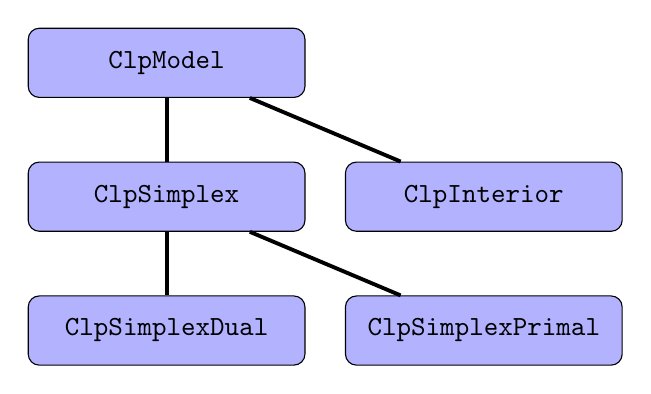
\begin{tikzpicture}[node distance=2.5cm]
    \tikzstyle{every state}=[rectangle,
                             minimum width=10em,
                             rounded corners,
                             fill=blue!30,
                             edge from parent,
                             text=black]
    \tikzset{node distance=1.7cm};

    \node[state] (a)                    {\texttt{ClpModel}};
    \node[state] (b) [below of = a]     {\texttt{ClpSimplex}};
    \node[state] (c) [right = 0.5cm of b] {\texttt{ClpInterior}};
    \node[state] (d) [below of = b]     {\texttt{ClpSimplexDual}};
    \node[state] (e) [right = 0.5cm of d] {\texttt{ClpSimplexPrimal}};

    \tikzset{edgestyle/.style={-, double=black}}
%    \tikzset{every node/.style={fill=white}}

    \path (a) edge [edgestyle] node {}  (b)
          (a) edge [edgestyle] node {}  (c)
          (b) edge [edgestyle] node {}  (d)
          (b) edge [edgestyle] node {}  (e);
\end{tikzpicture}
\caption{Class hierarchy for \texttt{ClpModel}}
\label{fig:clpmodel}
\end{figure}


\section{Slp}
While implementing an algorithm, it makes sense to start to implement
sub-functions that are not dependant on other functions. 

Implementing the Taylor series expansion is pretty straight forward, as
we have a closed-form definition for the specific objective function that
we described in Chapter \ref{ch:qp}. The function prototype for the
Taylor series expansion reads:
\begin{verbatim}
void taylor(double* T, const double* x,
            const ClpModel& m);
\end{verbatim}
where \texttt{ClpModel} gives us access to both the linear and quadratic
objective term. The result of the Taylor-series expansion, i.e. the new
objective function, is put in \texttt{T}.

The next step in the Slp algorithm is to solve the new linear program with the
new objective function \texttt{T}. This is simply done with a call to Clp.

After solving the linear program, the next step is to find the one-dimensional
minimizer between our current point and the solution to the linear program we
just solved.
The step length $\alpha_k$ tells us where this minimizer lies between the two
points.
To implement this line search, we find a closed-form definition of the step
length $\alpha_k$ by letting $m(\alpha) = f((1-\alpha) x_k + \alpha \hat{x}_k)$
and setting $m^\prime(\alpha) = 0$ and solving for $\alpha$:
\[
\alpha_k = \frac{
                2x_k^T H x_k
                - 2\hat{x}_k^T H x_k
                + b^T x_k - b^T \hat{x}_k
                }{
                  2\hat{x}_k^T H \hat{x}_k
                - 4\hat{x}_k^T H x_k
                + 2x_k^T H x_k
                }
\]
The function prototype for the line search function reads:
\begin{verbatim}
double lineSearch(const double* p,
                  const double* q,
                  ClpModel& m);
\end{verbatim}
where \texttt{ClpModel} gives us access to both the linear and quadratic
objective term.

The termination condition of Slp depends on the objective value of the two
previous iterations. So, in order to terminate, we need a function that can
compute the objective value. The function prototype for this function reads:
\begin{verbatim}
double objVal(const double* p, const ClpModel& m);
\end{verbatim}
where \texttt{ClpModel} again gives us access to both the linear and quadratic
objective term.

These three functions all have an asymptotic running time in the order of the
number of columns in the problem, because they do a constant number of
operations while iterating sparsely through matrix $H$ and vector $b$.

When it comes to decisions to be made around data types and storage formats,
there is not really too much to be said, because the choices are quite limited.
It is pretty much dependant on the linear programming solver that is used.
As mentioned earlier, Clp stores matrices in a sparse format, and all the sub
functions only operate on non-zero elements, so there is not really room for
much overhead.

An implementation of Algorithm \ref{alg:iter} in \texttt{C++} looks like this:
\begin{verbatim}
ClpModel lin = m; // A linear copy of ClpModel m
do {
    taylor(T, x, m);

    lin.chgObjCoefficients(T); // Set new linear objective
    lin.primal(); // Run the primal simplex method
    
    const double* xhat = lin.primalColumnSolution(); // Opt. sol
    double alpha = lineSearch(x, xhat, m);
    if      (alpha > 1) alpha = 1;
    else if (alpha < 0) alpha = 0;

    double oldval = objVal(x, m);
    for (int i = 0; i < numCols; i++) {
        x[i] = (1-alpha) * xhat[i];
    }
    double val = objVal(x, m);

    stop = (oldval - val);
    stop /= fabs(oldval);
} while (stop > tolerance);
\end{verbatim}


\section{Solving Subinstances}
In this section, we discuss the implementation of the different approaches to
solving several subinstances.
As mentioned in the beginning of the chapter, the two
main approaches are to solve a limited amount of subinstances, bounded
by $\sigma(\beta, n)$ for some $\beta$ and a problem size $n$, or to implement a discrete
event simulator that only stores the current state of the network.
First we will discuss the implementation of the tree structure, before we
move on to the two main approaches.

\subsection{Tree Structure}
All trees consists of vertices, and in our specific case, each vertex contains
two sets $\mathcal{M}$ and $\mathcal{Z}$, a solution $x^*$, and a number of
child vertices. To keep vertices as simple as possible, we implement them as
simple \texttt{structs}. Each vertex \texttt{struct} looks like
this:
\begin{verbatim}
struct vertex {
  set<uint16_t> m;
  set<uint16_t> z;
  double* sol;
  vector<struct vertex*> children;
};
\end{verbatim}
A reader familiar with \texttt{C++} might notice that we use
\texttt{set} instead of using a bit vector as we discussed
in Section \ref{ch:tree}, and we will come to that later. Note that
the sets consist of indices of primitive type \texttt{uint16\_t}, which is
short for \texttt{unsigned short int}. That means that the sets are limited to
$2^{16} = 65536$ elements, and therefore also putting a limit to the size
of the QP problems that can be solved. This seems like a reasonable limit
as Goodtech wants to solve problems with $200 - 2000$ variables.
If they need to solve larger problems in the future, it is possible to change
the primitive data type.

As soon as a vertex is defined, we are ready to implement \texttt{mfind}.
Remember that \texttt{mfind} is a modified version of \texttt{find} that tells
us which vertex should be the parent of our potentially new vertex in case it
has a distinct solution.
\texttt{mfind} is defined in two parts. The first part is a driver function
for starting the algorithm on some vertex. The second part is the actual
recursively defined algorithm. These two parts are called \texttt{mfind} and
\texttt{mfindrec}, respectively. We define \texttt{mfind} as follows:
\begin{verbatim}
bool mfind(const set<uint16_t>& m,
struct vertex* v, struct vertex*& ret)
{
  ret = v;
  return mfindrec(m, v, ret);
}
\end{verbatim}
The parameters for \texttt{mfind} are a modifier, a vertex where the search
will begin and an output vertex.
In order to search the whole tree, one would use the root vertex as parameter
\texttt{v}.
The function returns a boolean that changes the meaning of the output vertex.
The function makes a call to \texttt{mfindrec}:
\begin{verbatim}
bool mfindrec(const std::set<uint16_t>& m,
struct vertex* v, struct vertex*& ret)
{
  if (isSubset(m, v->z)) return true;
  for (struct vertex* vi : v->children) {
    if (isSubset(vi->m, m)) {
      ret = vi; 
      bool temp = mfindrec(m, vi, ret);
      if (temp) return true;
    }   
  }   
  return false;
}
\end{verbatim}
It is quite evident from the code that the performance of the \texttt{isSubset}
function is important. In Chapter \ref{ch:tree} we discussed using bit vectors 
to represent sets. We concluded that a simple \texttt{AND} operation would tell
us whether a set was a subset of another set.
We also discussed the possibility of it being more memory efficient than
storing sets in a sparse format where only the indices of each variable was
stored.

Using a bit vector, each set consumes exactly $n$ bits of storage if our
\emph{universe} holds $n$ variables.
Using sets of sparsely stored indices, each set consumes a varying amount of
bits depending on how many variables are in the set. If each index is of data
type \texttt{uint16\_t}, then each index consumes $16$ bits. The trade-off
here is quite clear: If a set contains less than one sixteenth of $n$, then
the sparse format uses less memory. This might actually be the case in a lot
of sets, especially when solving all possible subinstances where the number
of breakdowns are limited by some $\beta$. Consider a very small case where
$n = 200$ and we solve all subinstances
$\sigma(3, 200) = \sum_{j=0}^{3} {\binom{200}{j}} = S$.
With a total number of $S$ sets stored as bit vectors, the memory use for
storing the modifiers is $200S~\textrm{bits} \approx 32~\textrm{megabytes}$.
Whereas, with $S$ sets of sparsely stored indices, the memory use for storing
the modifiers is approximately $8$ megabytes. However, as $\beta$ increases,
the greater the benefits of storing sets in bit vectors become evident. As soon
as $\beta$ becomes greater than 12, bit vectors will use less memory to store all
modifiers. Figure \ref{fig:bmem} shows the ratio of memory used by bit vectors
over memory used by sets of sparsely stored indices where $n = 200$ and
$5 \leq \beta \leq 30$.
\begin{figure}[ht!]
\centering
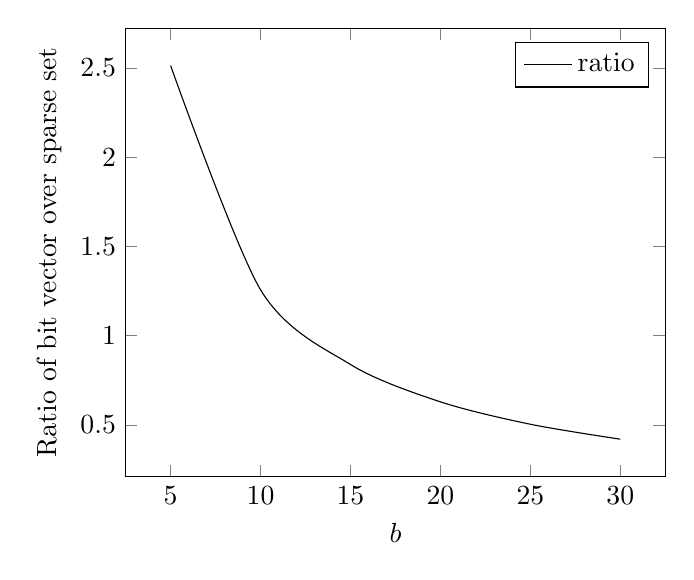
\begin{tikzpicture}
    \begin{axis}[
        legend pos=north east,
        xlabel=$b$,
        ylabel=Ratio of bit vector over sparse set]

        \addplot[black, smooth] plot coordinates {
            (5,  2.51302)
            (10, 1.25686)
            (15, 0.838169)
            (20, 0.628847)
            (25, 0.503276)
            (30, 0.419585)
        };

        \legend{ratio}
    \end{axis}
\end{tikzpicture}

\caption{The ratio of memory use of \texttt{bitset} over \texttt{set} as a
         function of $\beta$.}
\label{fig:bmem}
\end{figure}
Aside from the modifier set, we also have to store the set of variables that
are equal to zero in the optimal solutions of each subinstance. These sets
are more difficult to analyze in terms of memory use, simply because the
cardinality is unknown. However, we do know that $|\mathcal{Z}_k| \geq
|\mathcal{M}_k|$.

With sets of sparsely stored indices, we only need to check the variables
that are actually in the sets in order to determine if a set is a subset
of some set. However, with bit vectors, we need to check $n$ bits---where $n$
is the number of variables in the universe---in order to determine the same.
This means that the \texttt{isSubset} routine will most likely have a different
running time with the two implementations.

One way to find out which of the two are most suited for our need is to perform
a benchmark of the two.
By setting the universe to some size $n$, and generating sets of
random sparsity less than or equal to $n$, we can test how fast
\texttt{isSubset} will run.
We generate random sets as \texttt{bitsets} in \texttt{C++}, storing copies
of these sets in the sparse representation, then testing the performance 
of both implementations of \texttt{isSubset}.
Figure \ref{fig:setspeed}
shows the running time of the two implementations in seconds. Both
implementations were tested on $3000^2$ \texttt{isSubset}-executions, while
increasing $n$.
Codes for the benchmark can be found in Appendix \ref{app:setbench}.
\begin{figure}[ht!]
\centering
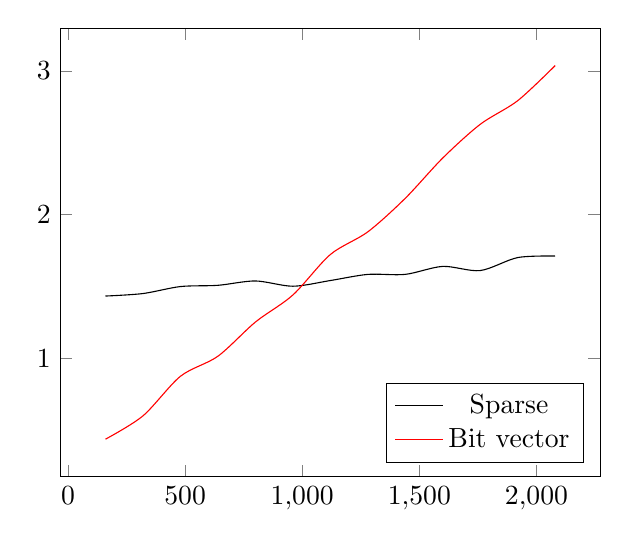
\begin{tikzpicture}
    \begin{axis}[
        legend pos=south east]
%        xlabel=Variables in Universe,
%        ylabel=Seconds]

        \addplot[black, smooth] plot coordinates {
(160, 1.43344)
(320, 1.45082)
(480, 1.49948)
(640, 1.50815)
(800, 1.53846)
(960, 1.50186)
(1120, 1.54138)
(1280, 1.58404)
(1440, 1.58431)
(1600, 1.63973)
(1760, 1.61084)
(1920, 1.70125)
(2080, 1.71173)
        };

        \addplot[red, smooth] plot coordinates {
(160, 0.437256)
(320, 0.599489)
(480, 0.875034)
(640, 1.01462)
(800, 1.25228)
(960, 1.44069)
(1120, 1.72237)
(1280, 1.88017)
(1440, 2.11386)
(1600, 2.39418)
(1760, 2.6287)
(1920, 2.79312)
(2080, 3.03735)
        };

        \legend{Sparse, Bit vector}
    \end{axis}
\end{tikzpicture}

\caption{CPU-seconds used to execute $3000^2$ calls to \texttt{isSubset} on
         randomly generated sets with random sparsity as a function of $n$.}
\label{fig:setspeed}
\end{figure}

We see that the bit vector implementation is much faster than the sparse
implementation on smaller universes. However, the sparse implementation
scales much better than the bit vector implementation when the size of
the universe increases. When it comes to memory, the situation is the same,
except reversed. The sets of sparsely stored indices obviously uses less
memory when $\beta$ is small, i.e. the modifiers are more sparse. However, they
do not scale as nicely as the bit vectors. So the choice relies on what is
most important: memory or speed. Since the nature of this thesis is to
implement a \emph{fast} solver, we give speed a higher priority than memory 
efficiency, so we choose to implement the sets of sparsely stored
indices. That is, in \texttt{C++}, \texttt{set}.

\subsection{Tree Construction}
Because we do not need to store any information about edges in the tree,
we do not need to implement edges as an object of its own. We defined
a vertex \texttt{struct} earlier, having a \texttt{vector} of child
vertices. That means that for each vertex we have, we can reach all child
vertices, children's child vertices and so on, from that vertex.
So, if we have a pointer to the root of a tree, we can reach all vertices
in the tree. Although we earlier defined a tree as an ordered pair
$(V, E)$ of a set of vertices $V$ and a set of edges $E$, we only need a
pointer \texttt{struct vertex*} to our root to access our tree.

The biggest operations in Algorithm \ref{alg:construct} is iterating the power
set of $\left\{1,2,\ldots,n\right\}$. There are lots of combination generators available, so
instead of re-inventing the wheel, we choose a generator that suits our needs.
We need one that is easy to use, and is capable of generating combinations of
a given cardinality. One implementation, similar in use to
\texttt{next\_permutation} in the standard \texttt{C++ STL}, is presented
in~\cite{codeproject}.
Codes from \cite{codeproject} can be found in Appendix
\ref{app:nextcombination}.

The remaining parts of the \texttt{construct}-routine is just running
\texttt{mfind} on each generated modifier, and adding it to the tree
if necessary. Then at the end, return the pointer to the root vertex.

\subsection{Discrete Event Simulation}
In a discrete event simulation (DES), operations are always triggered by events.
In a DES for the reliability analyses discussed in Chapter \ref{ch:intro},
we only need to consider two types of events; a breakdown in the network,
or that a link is repaired.
Each link in the network is represented by
a variable, so each event can by represented by a single variable.

The current state of our system is easily represented by a QP $\mathcal{Q}$ and
a set of variables representing the current broken links in our network.
As this set represents broken links, just like our modifiers $\mathcal{M}_k$
represents breakdowns, we choose to denote the current state of the system
by $\mathcal{M}$. 

Given a variable $x$ to represent a link that breaks down, we need to
update the  current state of the system. This is done with a simple
\textit{union}
\[
\mathcal{M} = \mathcal{M} \cup \left\{x\right\}.
\]
Given a variable $x$ of variables to represent a repaired link, we update the
current state with a simple \textit{relative complement}
\[
\mathcal{M} = \mathcal{M} \setminus \left\{x\right\}.
\]
We call these two operations for \texttt{break} and \texttt{repair}, respectively.
After every change of state in the system, we need to solve the subinstance
of $\mathcal{Q}$ defined by the modifier $\mathcal{M}$.

As the state of the system changes, we need to solve more and more subinstances.
We can choose whether or not we want to store the modifiers and their respective
solutions in a tree or not. If we choose to store distinct solutions in a tree,
we check the tree for a solution for the subinstance defined by the newly
updated modifier, before we potentially solve the problem.


\section{A Quick Overview}
In this section we present a quick overview of the different
implementations.

Although Clp is written primarily for solving linear
programs, it comes with a QP solver. This QP solver uses an implementation
of a primal-dual predictor-corrector interior point method. In addition
to Clp's QP solver, we also have the QP solver presented in Section
\ref{ch:slp}.

There are four different implementations we have, named
\texttt{construct\_clp}, \texttt{construct\_slp}, \texttt{naive\_clp} and
\texttt{naive\_slp}. The implementations with names ending with
\texttt{\_clp} and \texttt{\_slp} uses Clp's QP solver and Slp, respectively,
whenever a QP needs to be solved.
The \texttt{construct} implementations uses the tree structured presented
in Section \ref{ch:tree} for storing subinstances with distinct solutions.
The \texttt{naive} implementations, however, solves subinstances regardless of
whether they have distinct solutions or not.

In the next section, we present several experiments to perform on our
implementations.

\chapter{Implementation}
Recall from Chapter \ref{ch:qp} that we discussed limiting the amount
of subinstances to solve. We did this by introducing a limit on the number of
simultaneous break-downs in the network by some $\beta$.
Another approach is to implement a discrete-event simulator (DES). Each event
occurs at a particular instant in time that changes the state of the system.
In this case, each event would either be a breakdown in the network, or that
a breakdown is fixed.

The difference in these two approaches are prominent, but they share the same
core, namely a QP solver. In this chapter we first discuss the implementation
of the solver declared in Chapter \ref{ch:slp}, before we move on to the
implementation of the two approaches of solving several subinstances.
\label{ch:implementation}

\section{Finding an LP Solver}
The method described in Chapter \ref{ch:slp} relies on repetitively solving
linear programs. Before implementing such a method, it is important to choose
an appropriate LP solver. The solver must
\begin{inparaenum}[\itshape a\upshape)]
\item be released under a free license; and
\item it must allow library calls in C/C++
\end{inparaenum}

Among a list of about 50 solvers (most of them proprietary), the
following three matches the aforementioned criteria:
\begin{description}
\item[Clp] \hfill \\
Clp is short for Coin-or linear programming. It is a free linear programming
solver released under the Common Public License (CPL). It is primarily meant to
be used as a callable library. Its license allows other software to link to the
Clp library without requiring that that software is released under the same
license (permissive). \cite{clp}
\item[GLPK] \hfill \\
GLPK is short for GNU Linear Programming Kit. It is a free linear (integer)
programming software packaged released under the GNU General Public License
(GNU GPL). GLPK is organized in the form of a callable library. Its license
requires linking software to be released under the GNU GPL (reciprocal).
\cite{glpk}
\item[lp\_solve] \hfill \\
lp\_solve is a free linear (integer) programming solver released under the GNU 
Lesser General Public License (GNU LGPL). Its license is permissive like the
CPL. \cite{lpsolve}
\end{description}

Incidentally, these tree solvers are the only three open source LP solvers
suggested by the NEOS Optimization Guide~\cite{neos}.
In addition to the mentioned criteria, it is important that the solver is
fast.
Moreover, it needs to be fast on problems that fit the description in
Section \ref{sec:problem}.

Testing the three solvers on linearized versions of the instances
\textit{small} and \textit{large}---presented in
Chapter \ref{sec:instances}---reveals the running times shown in Table
\ref{table:lpres}.
The running times are the number of seconds in CPU-time after 1000 runs.

\begin{table}[ht!]
    \centering
    \caption{Running time in CPU-seconds used by each solver to solve 1000
             instances of each problem.}
    \begin{tabular}{lrrr}
        Data Set       & Clp    & GLPK   & lp\_solve \\ \hline
        \textit{small} & 6.929  & 26.096 & 4.734 \\
        \textit{large} & 12.832 & 47.977 & 23.376
    \end{tabular}
    \label{table:lpres}
\end{table}

While lp\_solve is the fastest on a smaller LP, it doesn't scale as well as
with larger problems like Clp does.

GoodTech need to solve problems with more than 200 variables, and
\textit{small} is almost hitting that lower limit, so a good result on
\textit{large} is prioritized over the other.
This means that Clp outperforms the other two solvers in this test.

Although this is not an extensive test, it is a pretty good indicator that Clp
will be the fastest solver on similar problems.


\section{Clp}
Clp is written primarily by John J. Forrest, now retired from IBM Research. At
the time of writing, Clp is under active development. It is currently
managed by John Forrest, Julian Hall, Lou Hafer and Matthew Saltzman.
\cite{clppage}

Matrices in Clp are stored in a compact format using three vectors.
The first vector contains all the non-zero elements of the matrix.
The second vector contains the indices of the elements in the first vector.
The third vector contains an accumulated number of elements in each row/column.
The order of the elements depends whether the matrix is row-ordered or
column-ordered.
The indices represent the column/row position of the elements, and the
accumulated values represent the accumulated number of elements in the
row/columns depending on whether the matrix is row-ordered or column-ordered,
respectively.
To get a better understanding of how they are stored, consider the matrix
\[
\left[
\begin{array}{rrrrrrrr}
    3 & 1 & 0   & -2  & -1 & 0 & 0    & -1 \\
    0 & 2 & 1.1 & 0   & 0  & 0 & 0    & 0  \\
    0 & 0 & 1   & 0   & 0  & 1 & 0    & 0  \\
    0 & 0 & 0   & 2.8 & 0  & 0 & -1.2 & 0  \\
  5.6 & 0 & 0   & 0   & 1  & 0 & 0    & 1.9  

\end{array}
\right]
\]
being stored in row-ordered format, then the element vector would be
\[
\begin{array}{l}
\left[
\begin{array}{rrrrrrr}
    3 & 1 & -2 & -1 & -1 & 2 & 1.1
\end{array}\right. \\
\left.\begin{array}{rrrrrrr}
    1 & 1 & 2.8 & -1.2 & 5.6 & 1 & 1.9
\end{array}
\right]^T,
\end{array}
\]
the vector containing the column indices would be
\[
\left[
\begin{array}{rrrrrrrrrrrrrr}
    0 & 1 & 3 & 4 & 7 & 1 & 2 & 2 & 5 & 3 & 6 & 0 & 4 & 7
\end{array}
\right]^T,
\]
and the vector containing the vector starts (the accumulated indices) would be
\[
\left[
\begin{array}{rrrrrr}
    0 & 5 & 7 & 9 & 11 & 14
\end{array}
\right]^T.
\]
The \texttt{CoinPackedMatrix} class represents such a compact matrix.
To keep overhead at a minimum, it is important to implement the new solver
(from here on called Slp) using the same compact format.

Clp has a base class that holds data for both linear and quadratic models
called \texttt{ClpModel}.
The class itself knows nothing about the implementation of the algorithms, but
it contains all the data about a problem needed to apply an algorithm on that
data.
This is very handy for passing data throughout Slp without much overhead.
It also results in very neat function prototypes as only one parameter
is needed for passing lots of information. For instance, the function prototype
in Slp for the function that performs the line search described in Chapter
\ref{ch:slp} looks like this:
\begin{verbatim}
double lineSearch(const double* a,
                  const double* b,
                  ClpModel& m);
\end{verbatim}
Figure \ref{fig:clpmodel} shows the class hierarchy for \texttt{ClpModel}.
The subclasses contain the implementation of the algorithms that their class
names describe. For instance, \texttt{ClpSimplexDual} contains the
implementation of the Dual Simplex Algorithm.
\begin{figure}
\centering
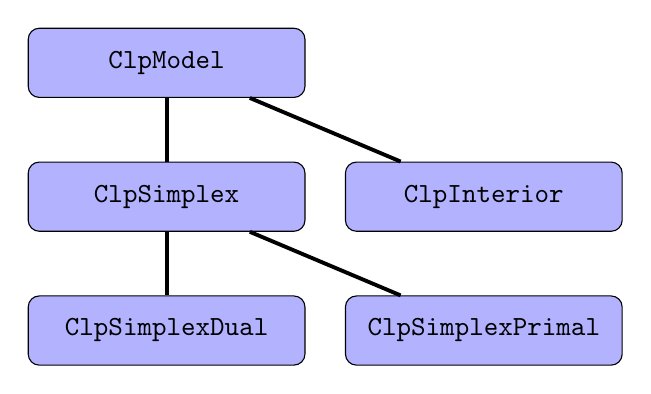
\begin{tikzpicture}[node distance=2.5cm]
    \tikzstyle{every state}=[rectangle,
                             minimum width=10em,
                             rounded corners,
                             fill=blue!30,
                             edge from parent,
                             text=black]
    \tikzset{node distance=1.7cm};

    \node[state] (a)                    {\texttt{ClpModel}};
    \node[state] (b) [below of = a]     {\texttt{ClpSimplex}};
    \node[state] (c) [right = 0.5cm of b] {\texttt{ClpInterior}};
    \node[state] (d) [below of = b]     {\texttt{ClpSimplexDual}};
    \node[state] (e) [right = 0.5cm of d] {\texttt{ClpSimplexPrimal}};

    \tikzset{edgestyle/.style={-, double=black}}
%    \tikzset{every node/.style={fill=white}}

    \path (a) edge [edgestyle] node {}  (b)
          (a) edge [edgestyle] node {}  (c)
          (b) edge [edgestyle] node {}  (d)
          (b) edge [edgestyle] node {}  (e);
\end{tikzpicture}
\caption{Class hierarchy for \texttt{ClpModel}}
\label{fig:clpmodel}
\end{figure}


\section{Slp}
While implementing an algorithm, it makes sense to start to implement
sub-functions that are not dependant on other functions. 

Implementing the Taylor series expansion is pretty straight forward, as
we have a closed-form definition for the specific objective function that
we described in Chapter \ref{ch:qp}. The function prototype for the
Taylor series expansion reads:
\begin{verbatim}
void taylor(double* T, const double* x,
            const ClpModel& m);
\end{verbatim}
where \texttt{ClpModel} gives us access to both the linear and quadratic
objective term. The result of the Taylor-series expansion, i.e. the new
objective function, is put in \texttt{T}.

The next step in the Slp algorithm is to solve the new linear program with the
new objective function \texttt{T}. This is simply done with a call to Clp.

After solving the linear program, the next step is to find the one-dimensional
minimizer between our current point and the solution to the linear program we
just solved.
The step length $\alpha_k$ tells us where this minimizer lies between the two
points.
To implement this line search, we find a closed-form definition of the step
length $\alpha_k$ by letting $m(\alpha) = f((1-\alpha) x_k + \alpha \hat{x}_k)$
and setting $m^\prime(\alpha) = 0$ and solving for $\alpha$:
\[
\alpha_k = \frac{
                2x_k^T H x_k
                - 2\hat{x}_k^T H x_k
                + b^T x_k - b^T \hat{x}_k
                }{
                  2\hat{x}_k^T H \hat{x}_k
                - 4\hat{x}_k^T H x_k
                + 2x_k^T H x_k
                }
\]
The function prototype for the line search function reads:
\begin{verbatim}
double lineSearch(const double* p,
                  const double* q,
                  ClpModel& m);
\end{verbatim}
where \texttt{ClpModel} gives us access to both the linear and quadratic
objective term.

The termination condition of Slp depends on the objective value of the two
previous iterations. So, in order to terminate, we need a function that can
compute the objective value. The function prototype for this function reads:
\begin{verbatim}
double objVal(const double* p, const ClpModel& m);
\end{verbatim}
where \texttt{ClpModel} again gives us access to both the linear and quadratic
objective term.

These three functions all have an asymptotic running time in the order of the
number of columns in the problem, because they do a constant number of
operations while iterating sparsely through matrix $H$ and vector $b$.

When it comes to decisions to be made around data types and storage formats,
there is not really too much to be said, because the choices are quite limited.
It is pretty much dependant on the linear programming solver that is used.
As mentioned earlier, Clp stores matrices in a sparse format, and all the sub
functions only operate on non-zero elements, so there is not really room for
much overhead.

An implementation of Algorithm \ref{alg:iter} in \texttt{C++} looks like this:
\begin{verbatim}
ClpModel lin = m; // A linear copy of ClpModel m
do {
    taylor(T, x, m);

    lin.chgObjCoefficients(T); // Set new linear objective
    lin.primal(); // Run the primal simplex method
    
    const double* xhat = lin.primalColumnSolution(); // Opt. sol
    double alpha = lineSearch(x, xhat, m);
    if      (alpha > 1) alpha = 1;
    else if (alpha < 0) alpha = 0;

    double oldval = objVal(x, m);
    for (int i = 0; i < numCols; i++) {
        x[i] = (1-alpha) * xhat[i];
    }
    double val = objVal(x, m);

    stop = (oldval - val);
    stop /= fabs(oldval);
} while (stop > tolerance);
\end{verbatim}


\section{Solving Subinstances}
In this section, we discuss the implementation of the different approaches to
solving several subinstances.
As mentioned in the beginning of the chapter, the two
main approaches are to solve a limited amount of subinstances, bounded
by $\sigma(\beta, n)$ for some $\beta$ and a problem size $n$, or to implement a discrete
event simulator that only stores the current state of the network.
First we will discuss the implementation of the tree structure, before we
move on to the two main approaches.

\subsection{Tree Structure}
All trees consists of vertices, and in our specific case, each vertex contains
two sets $\mathcal{M}$ and $\mathcal{Z}$, a solution $x^*$, and a number of
child vertices. To keep vertices as simple as possible, we implement them as
simple \texttt{structs}. Each vertex \texttt{struct} looks like
this:
\begin{verbatim}
struct vertex {
  set<uint16_t> m;
  set<uint16_t> z;
  double* sol;
  vector<struct vertex*> children;
};
\end{verbatim}
A reader familiar with \texttt{C++} might notice that we use
\texttt{set} instead of using a bit vector as we discussed
in Section \ref{ch:tree}, and we will come to that later. Note that
the sets consist of indices of primitive type \texttt{uint16\_t}, which is
short for \texttt{unsigned short int}. That means that the sets are limited to
$2^{16} = 65536$ elements, and therefore also putting a limit to the size
of the QP problems that can be solved. This seems like a reasonable limit
as Goodtech wants to solve problems with $200 - 2000$ variables.
If they need to solve larger problems in the future, it is possible to change
the primitive data type.

As soon as a vertex is defined, we are ready to implement \texttt{mfind}.
Remember that \texttt{mfind} is a modified version of \texttt{find} that tells
us which vertex should be the parent of our potentially new vertex in case it
has a distinct solution.
\texttt{mfind} is defined in two parts. The first part is a driver function
for starting the algorithm on some vertex. The second part is the actual
recursively defined algorithm. These two parts are called \texttt{mfind} and
\texttt{mfindrec}, respectively. We define \texttt{mfind} as follows:
\begin{verbatim}
bool mfind(const set<uint16_t>& m,
struct vertex* v, struct vertex*& ret)
{
  ret = v;
  return mfindrec(m, v, ret);
}
\end{verbatim}
The parameters for \texttt{mfind} are a modifier, a vertex where the search
will begin and an output vertex.
In order to search the whole tree, one would use the root vertex as parameter
\texttt{v}.
The function returns a boolean that changes the meaning of the output vertex.
The function makes a call to \texttt{mfindrec}:
\begin{verbatim}
bool mfindrec(const std::set<uint16_t>& m,
struct vertex* v, struct vertex*& ret)
{
  if (isSubset(m, v->z)) return true;
  for (struct vertex* vi : v->children) {
    if (isSubset(vi->m, m)) {
      ret = vi; 
      bool temp = mfindrec(m, vi, ret);
      if (temp) return true;
    }   
  }   
  return false;
}
\end{verbatim}
It is quite evident from the code that the performance of the \texttt{isSubset}
function is important. In Chapter \ref{ch:tree} we discussed using bit vectors 
to represent sets. We concluded that a simple \texttt{AND} operation would tell
us whether a set was a subset of another set.
We also discussed the possibility of it being more memory efficient than
storing sets in a sparse format where only the indices of each variable was
stored.

Using a bit vector, each set consumes exactly $n$ bits of storage if our
\emph{universe} holds $n$ variables.
Using sets of sparsely stored indices, each set consumes a varying amount of
bits depending on how many variables are in the set. If each index is of data
type \texttt{uint16\_t}, then each index consumes $16$ bits. The trade-off
here is quite clear: If a set contains less than one sixteenth of $n$, then
the sparse format uses less memory. This might actually be the case in a lot
of sets, especially when solving all possible subinstances where the number
of breakdowns are limited by some $\beta$. Consider a very small case where
$n = 200$ and we solve all subinstances
$\sigma(3, 200) = \sum_{j=0}^{3} {\binom{200}{j}} = S$.
With a total number of $S$ sets stored as bit vectors, the memory use for
storing the modifiers is $200S~\textrm{bits} \approx 32~\textrm{megabytes}$.
Whereas, with $S$ sets of sparsely stored indices, the memory use for storing
the modifiers is approximately $8$ megabytes. However, as $\beta$ increases,
the greater the benefits of storing sets in bit vectors become evident. As soon
as $\beta$ becomes greater than 12, bit vectors will use less memory to store all
modifiers. Figure \ref{fig:bmem} shows the ratio of memory used by bit vectors
over memory used by sets of sparsely stored indices where $n = 200$ and
$5 \leq \beta \leq 30$.
\begin{figure}[ht!]
\centering
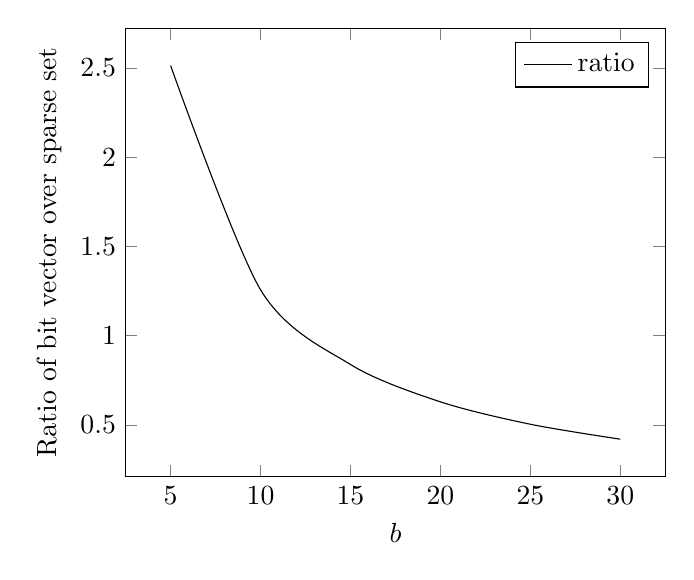
\begin{tikzpicture}
    \begin{axis}[
        legend pos=north east,
        xlabel=$b$,
        ylabel=Ratio of bit vector over sparse set]

        \addplot[black, smooth] plot coordinates {
            (5,  2.51302)
            (10, 1.25686)
            (15, 0.838169)
            (20, 0.628847)
            (25, 0.503276)
            (30, 0.419585)
        };

        \legend{ratio}
    \end{axis}
\end{tikzpicture}

\caption{The ratio of memory use of \texttt{bitset} over \texttt{set} as a
         function of $\beta$.}
\label{fig:bmem}
\end{figure}
Aside from the modifier set, we also have to store the set of variables that
are equal to zero in the optimal solutions of each subinstance. These sets
are more difficult to analyze in terms of memory use, simply because the
cardinality is unknown. However, we do know that $|\mathcal{Z}_k| \geq
|\mathcal{M}_k|$.

With sets of sparsely stored indices, we only need to check the variables
that are actually in the sets in order to determine if a set is a subset
of some set. However, with bit vectors, we need to check $n$ bits---where $n$
is the number of variables in the universe---in order to determine the same.
This means that the \texttt{isSubset} routine will most likely have a different
running time with the two implementations.

One way to find out which of the two are most suited for our need is to perform
a benchmark of the two.
By setting the universe to some size $n$, and generating sets of
random sparsity less than or equal to $n$, we can test how fast
\texttt{isSubset} will run.
We generate random sets as \texttt{bitsets} in \texttt{C++}, storing copies
of these sets in the sparse representation, then testing the performance 
of both implementations of \texttt{isSubset}.
Figure \ref{fig:setspeed}
shows the running time of the two implementations in seconds. Both
implementations were tested on $3000^2$ \texttt{isSubset}-executions, while
increasing $n$.
Codes for the benchmark can be found in Appendix \ref{app:setbench}.
\begin{figure}[ht!]
\centering
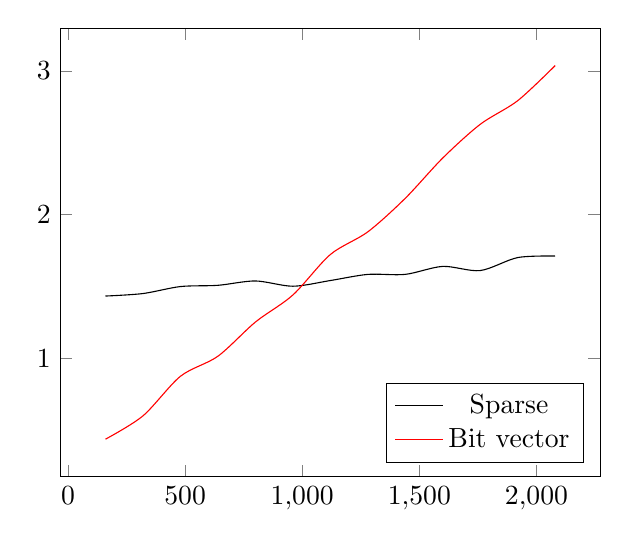
\begin{tikzpicture}
    \begin{axis}[
        legend pos=south east]
%        xlabel=Variables in Universe,
%        ylabel=Seconds]

        \addplot[black, smooth] plot coordinates {
(160, 1.43344)
(320, 1.45082)
(480, 1.49948)
(640, 1.50815)
(800, 1.53846)
(960, 1.50186)
(1120, 1.54138)
(1280, 1.58404)
(1440, 1.58431)
(1600, 1.63973)
(1760, 1.61084)
(1920, 1.70125)
(2080, 1.71173)
        };

        \addplot[red, smooth] plot coordinates {
(160, 0.437256)
(320, 0.599489)
(480, 0.875034)
(640, 1.01462)
(800, 1.25228)
(960, 1.44069)
(1120, 1.72237)
(1280, 1.88017)
(1440, 2.11386)
(1600, 2.39418)
(1760, 2.6287)
(1920, 2.79312)
(2080, 3.03735)
        };

        \legend{Sparse, Bit vector}
    \end{axis}
\end{tikzpicture}

\caption{CPU-seconds used to execute $3000^2$ calls to \texttt{isSubset} on
         randomly generated sets with random sparsity as a function of $n$.}
\label{fig:setspeed}
\end{figure}

We see that the bit vector implementation is much faster than the sparse
implementation on smaller universes. However, the sparse implementation
scales much better than the bit vector implementation when the size of
the universe increases. When it comes to memory, the situation is the same,
except reversed. The sets of sparsely stored indices obviously uses less
memory when $\beta$ is small, i.e. the modifiers are more sparse. However, they
do not scale as nicely as the bit vectors. So the choice relies on what is
most important: memory or speed. Since the nature of this thesis is to
implement a \emph{fast} solver, we give speed a higher priority than memory 
efficiency, so we choose to implement the sets of sparsely stored
indices. That is, in \texttt{C++}, \texttt{set}.

\subsection{Tree Construction}
Because we do not need to store any information about edges in the tree,
we do not need to implement edges as an object of its own. We defined
a vertex \texttt{struct} earlier, having a \texttt{vector} of child
vertices. That means that for each vertex we have, we can reach all child
vertices, children's child vertices and so on, from that vertex.
So, if we have a pointer to the root of a tree, we can reach all vertices
in the tree. Although we earlier defined a tree as an ordered pair
$(V, E)$ of a set of vertices $V$ and a set of edges $E$, we only need a
pointer \texttt{struct vertex*} to our root to access our tree.

The biggest operations in Algorithm \ref{alg:construct} is iterating the power
set of $\left\{1,2,\ldots,n\right\}$. There are lots of combination generators available, so
instead of re-inventing the wheel, we choose a generator that suits our needs.
We need one that is easy to use, and is capable of generating combinations of
a given cardinality. One implementation, similar in use to
\texttt{next\_permutation} in the standard \texttt{C++ STL}, is presented
in~\cite{codeproject}.
Codes from \cite{codeproject} can be found in Appendix
\ref{app:nextcombination}.

The remaining parts of the \texttt{construct}-routine is just running
\texttt{mfind} on each generated modifier, and adding it to the tree
if necessary. Then at the end, return the pointer to the root vertex.

\subsection{Discrete Event Simulation}
In a discrete event simulation (DES), operations are always triggered by events.
In a DES for the reliability analyses discussed in Chapter \ref{ch:intro},
we only need to consider two types of events; a breakdown in the network,
or that a link is repaired.
Each link in the network is represented by
a variable, so each event can by represented by a single variable.

The current state of our system is easily represented by a QP $\mathcal{Q}$ and
a set of variables representing the current broken links in our network.
As this set represents broken links, just like our modifiers $\mathcal{M}_k$
represents breakdowns, we choose to denote the current state of the system
by $\mathcal{M}$. 

Given a variable $x$ to represent a link that breaks down, we need to
update the  current state of the system. This is done with a simple
\textit{union}
\[
\mathcal{M} = \mathcal{M} \cup \left\{x\right\}.
\]
Given a variable $x$ of variables to represent a repaired link, we update the
current state with a simple \textit{relative complement}
\[
\mathcal{M} = \mathcal{M} \setminus \left\{x\right\}.
\]
We call these two operations for \texttt{break} and \texttt{repair}, respectively.
After every change of state in the system, we need to solve the subinstance
of $\mathcal{Q}$ defined by the modifier $\mathcal{M}$.

As the state of the system changes, we need to solve more and more subinstances.
We can choose whether or not we want to store the modifiers and their respective
solutions in a tree or not. If we choose to store distinct solutions in a tree,
we check the tree for a solution for the subinstance defined by the newly
updated modifier, before we potentially solve the problem.


\section{A Quick Overview}
In this section we present a quick overview of the different
implementations.

Although Clp is written primarily for solving linear
programs, it comes with a QP solver. This QP solver uses an implementation
of a primal-dual predictor-corrector interior point method. In addition
to Clp's QP solver, we also have the QP solver presented in Section
\ref{ch:slp}.

There are four different implementations we have, named
\texttt{construct\_clp}, \texttt{construct\_slp}, \texttt{naive\_clp} and
\texttt{naive\_slp}. The implementations with names ending with
\texttt{\_clp} and \texttt{\_slp} uses Clp's QP solver and Slp, respectively,
whenever a QP needs to be solved.
The \texttt{construct} implementations uses the tree structured presented
in Section \ref{ch:tree} for storing subinstances with distinct solutions.
The \texttt{naive} implementations, however, solves subinstances regardless of
whether they have distinct solutions or not.

In the next section, we present several experiments to perform on our
implementations.

\chapter{Implementation}
Recall from Chapter \ref{ch:qp} that we discussed limiting the amount
of subinstances to solve. We did this by introducing a limit on the number of
simultaneous break-downs in the network by some $\beta$.
Another approach is to implement a discrete-event simulator (DES). Each event
occurs at a particular instant in time that changes the state of the system.
In this case, each event would either be a breakdown in the network, or that
a breakdown is fixed.

The difference in these two approaches are prominent, but they share the same
core, namely a QP solver. In this chapter we first discuss the implementation
of the solver declared in Chapter \ref{ch:slp}, before we move on to the
implementation of the two approaches of solving several subinstances.
\label{ch:implementation}

\section{Finding an LP Solver}
The method described in Chapter \ref{ch:slp} relies on repetitively solving
linear programs. Before implementing such a method, it is important to choose
an appropriate LP solver. The solver must
\begin{inparaenum}[\itshape a\upshape)]
\item be released under a free license; and
\item it must allow library calls in C/C++
\end{inparaenum}

Among a list of about 50 solvers (most of them proprietary), the
following three matches the aforementioned criteria:
\begin{description}
\item[Clp] \hfill \\
Clp is short for Coin-or linear programming. It is a free linear programming
solver released under the Common Public License (CPL). It is primarily meant to
be used as a callable library. Its license allows other software to link to the
Clp library without requiring that that software is released under the same
license (permissive). \cite{clp}
\item[GLPK] \hfill \\
GLPK is short for GNU Linear Programming Kit. It is a free linear (integer)
programming software packaged released under the GNU General Public License
(GNU GPL). GLPK is organized in the form of a callable library. Its license
requires linking software to be released under the GNU GPL (reciprocal).
\cite{glpk}
\item[lp\_solve] \hfill \\
lp\_solve is a free linear (integer) programming solver released under the GNU 
Lesser General Public License (GNU LGPL). Its license is permissive like the
CPL. \cite{lpsolve}
\end{description}

Incidentally, these tree solvers are the only three open source LP solvers
suggested by the NEOS Optimization Guide~\cite{neos}.
In addition to the mentioned criteria, it is important that the solver is
fast.
Moreover, it needs to be fast on problems that fit the description in
Section \ref{sec:problem}.

Testing the three solvers on linearized versions of the instances
\textit{small} and \textit{large}---presented in
Chapter \ref{sec:instances}---reveals the running times shown in Table
\ref{table:lpres}.
The running times are the number of seconds in CPU-time after 1000 runs.

\begin{table}[ht!]
    \centering
    \caption{Running time in CPU-seconds used by each solver to solve 1000
             instances of each problem.}
    \begin{tabular}{lrrr}
        Data Set       & Clp    & GLPK   & lp\_solve \\ \hline
        \textit{small} & 6.929  & 26.096 & 4.734 \\
        \textit{large} & 12.832 & 47.977 & 23.376
    \end{tabular}
    \label{table:lpres}
\end{table}

While lp\_solve is the fastest on a smaller LP, it doesn't scale as well as
with larger problems like Clp does.

GoodTech need to solve problems with more than 200 variables, and
\textit{small} is almost hitting that lower limit, so a good result on
\textit{large} is prioritized over the other.
This means that Clp outperforms the other two solvers in this test.

Although this is not an extensive test, it is a pretty good indicator that Clp
will be the fastest solver on similar problems.


\section{Clp}
Clp is written primarily by John J. Forrest, now retired from IBM Research. At
the time of writing, Clp is under active development. It is currently
managed by John Forrest, Julian Hall, Lou Hafer and Matthew Saltzman.
\cite{clppage}

Matrices in Clp are stored in a compact format using three vectors.
The first vector contains all the non-zero elements of the matrix.
The second vector contains the indices of the elements in the first vector.
The third vector contains an accumulated number of elements in each row/column.
The order of the elements depends whether the matrix is row-ordered or
column-ordered.
The indices represent the column/row position of the elements, and the
accumulated values represent the accumulated number of elements in the
row/columns depending on whether the matrix is row-ordered or column-ordered,
respectively.
To get a better understanding of how they are stored, consider the matrix
\[
\left[
\begin{array}{rrrrrrrr}
    3 & 1 & 0   & -2  & -1 & 0 & 0    & -1 \\
    0 & 2 & 1.1 & 0   & 0  & 0 & 0    & 0  \\
    0 & 0 & 1   & 0   & 0  & 1 & 0    & 0  \\
    0 & 0 & 0   & 2.8 & 0  & 0 & -1.2 & 0  \\
  5.6 & 0 & 0   & 0   & 1  & 0 & 0    & 1.9  

\end{array}
\right]
\]
being stored in row-ordered format, then the element vector would be
\[
\begin{array}{l}
\left[
\begin{array}{rrrrrrr}
    3 & 1 & -2 & -1 & -1 & 2 & 1.1
\end{array}\right. \\
\left.\begin{array}{rrrrrrr}
    1 & 1 & 2.8 & -1.2 & 5.6 & 1 & 1.9
\end{array}
\right]^T,
\end{array}
\]
the vector containing the column indices would be
\[
\left[
\begin{array}{rrrrrrrrrrrrrr}
    0 & 1 & 3 & 4 & 7 & 1 & 2 & 2 & 5 & 3 & 6 & 0 & 4 & 7
\end{array}
\right]^T,
\]
and the vector containing the vector starts (the accumulated indices) would be
\[
\left[
\begin{array}{rrrrrr}
    0 & 5 & 7 & 9 & 11 & 14
\end{array}
\right]^T.
\]
The \texttt{CoinPackedMatrix} class represents such a compact matrix.
To keep overhead at a minimum, it is important to implement the new solver
(from here on called Slp) using the same compact format.

Clp has a base class that holds data for both linear and quadratic models
called \texttt{ClpModel}.
The class itself knows nothing about the implementation of the algorithms, but
it contains all the data about a problem needed to apply an algorithm on that
data.
This is very handy for passing data throughout Slp without much overhead.
It also results in very neat function prototypes as only one parameter
is needed for passing lots of information. For instance, the function prototype
in Slp for the function that performs the line search described in Chapter
\ref{ch:slp} looks like this:
\begin{verbatim}
double lineSearch(const double* a,
                  const double* b,
                  ClpModel& m);
\end{verbatim}
Figure \ref{fig:clpmodel} shows the class hierarchy for \texttt{ClpModel}.
The subclasses contain the implementation of the algorithms that their class
names describe. For instance, \texttt{ClpSimplexDual} contains the
implementation of the Dual Simplex Algorithm.
\begin{figure}
\centering
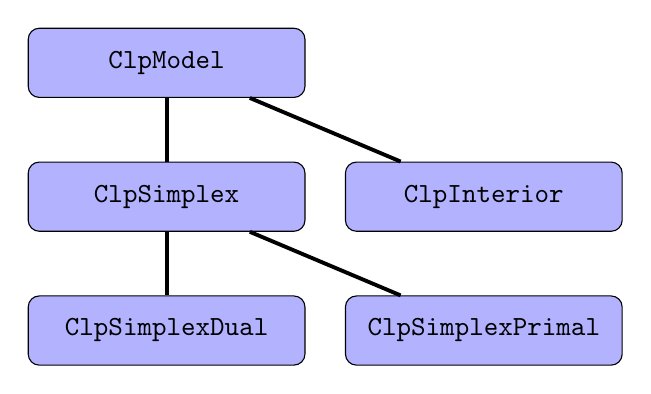
\begin{tikzpicture}[node distance=2.5cm]
    \tikzstyle{every state}=[rectangle,
                             minimum width=10em,
                             rounded corners,
                             fill=blue!30,
                             edge from parent,
                             text=black]
    \tikzset{node distance=1.7cm};

    \node[state] (a)                    {\texttt{ClpModel}};
    \node[state] (b) [below of = a]     {\texttt{ClpSimplex}};
    \node[state] (c) [right = 0.5cm of b] {\texttt{ClpInterior}};
    \node[state] (d) [below of = b]     {\texttt{ClpSimplexDual}};
    \node[state] (e) [right = 0.5cm of d] {\texttt{ClpSimplexPrimal}};

    \tikzset{edgestyle/.style={-, double=black}}
%    \tikzset{every node/.style={fill=white}}

    \path (a) edge [edgestyle] node {}  (b)
          (a) edge [edgestyle] node {}  (c)
          (b) edge [edgestyle] node {}  (d)
          (b) edge [edgestyle] node {}  (e);
\end{tikzpicture}
\caption{Class hierarchy for \texttt{ClpModel}}
\label{fig:clpmodel}
\end{figure}


\section{Slp}
While implementing an algorithm, it makes sense to start to implement
sub-functions that are not dependant on other functions. 

Implementing the Taylor series expansion is pretty straight forward, as
we have a closed-form definition for the specific objective function that
we described in Chapter \ref{ch:qp}. The function prototype for the
Taylor series expansion reads:
\begin{verbatim}
void taylor(double* T, const double* x,
            const ClpModel& m);
\end{verbatim}
where \texttt{ClpModel} gives us access to both the linear and quadratic
objective term. The result of the Taylor-series expansion, i.e. the new
objective function, is put in \texttt{T}.

The next step in the Slp algorithm is to solve the new linear program with the
new objective function \texttt{T}. This is simply done with a call to Clp.

After solving the linear program, the next step is to find the one-dimensional
minimizer between our current point and the solution to the linear program we
just solved.
The step length $\alpha_k$ tells us where this minimizer lies between the two
points.
To implement this line search, we find a closed-form definition of the step
length $\alpha_k$ by letting $m(\alpha) = f((1-\alpha) x_k + \alpha \hat{x}_k)$
and setting $m^\prime(\alpha) = 0$ and solving for $\alpha$:
\[
\alpha_k = \frac{
                2x_k^T H x_k
                - 2\hat{x}_k^T H x_k
                + b^T x_k - b^T \hat{x}_k
                }{
                  2\hat{x}_k^T H \hat{x}_k
                - 4\hat{x}_k^T H x_k
                + 2x_k^T H x_k
                }
\]
The function prototype for the line search function reads:
\begin{verbatim}
double lineSearch(const double* p,
                  const double* q,
                  ClpModel& m);
\end{verbatim}
where \texttt{ClpModel} gives us access to both the linear and quadratic
objective term.

The termination condition of Slp depends on the objective value of the two
previous iterations. So, in order to terminate, we need a function that can
compute the objective value. The function prototype for this function reads:
\begin{verbatim}
double objVal(const double* p, const ClpModel& m);
\end{verbatim}
where \texttt{ClpModel} again gives us access to both the linear and quadratic
objective term.

These three functions all have an asymptotic running time in the order of the
number of columns in the problem, because they do a constant number of
operations while iterating sparsely through matrix $H$ and vector $b$.

When it comes to decisions to be made around data types and storage formats,
there is not really too much to be said, because the choices are quite limited.
It is pretty much dependant on the linear programming solver that is used.
As mentioned earlier, Clp stores matrices in a sparse format, and all the sub
functions only operate on non-zero elements, so there is not really room for
much overhead.

An implementation of Algorithm \ref{alg:iter} in \texttt{C++} looks like this:
\begin{verbatim}
ClpModel lin = m; // A linear copy of ClpModel m
do {
    taylor(T, x, m);

    lin.chgObjCoefficients(T); // Set new linear objective
    lin.primal(); // Run the primal simplex method
    
    const double* xhat = lin.primalColumnSolution(); // Opt. sol
    double alpha = lineSearch(x, xhat, m);
    if      (alpha > 1) alpha = 1;
    else if (alpha < 0) alpha = 0;

    double oldval = objVal(x, m);
    for (int i = 0; i < numCols; i++) {
        x[i] = (1-alpha) * xhat[i];
    }
    double val = objVal(x, m);

    stop = (oldval - val);
    stop /= fabs(oldval);
} while (stop > tolerance);
\end{verbatim}


\section{Solving Subinstances}
In this section, we discuss the implementation of the different approaches to
solving several subinstances.
As mentioned in the beginning of the chapter, the two
main approaches are to solve a limited amount of subinstances, bounded
by $\sigma(\beta, n)$ for some $\beta$ and a problem size $n$, or to implement a discrete
event simulator that only stores the current state of the network.
First we will discuss the implementation of the tree structure, before we
move on to the two main approaches.

\subsection{Tree Structure}
All trees consists of vertices, and in our specific case, each vertex contains
two sets $\mathcal{M}$ and $\mathcal{Z}$, a solution $x^*$, and a number of
child vertices. To keep vertices as simple as possible, we implement them as
simple \texttt{structs}. Each vertex \texttt{struct} looks like
this:
\begin{verbatim}
struct vertex {
  set<uint16_t> m;
  set<uint16_t> z;
  double* sol;
  vector<struct vertex*> children;
};
\end{verbatim}
A reader familiar with \texttt{C++} might notice that we use
\texttt{set} instead of using a bit vector as we discussed
in Section \ref{ch:tree}, and we will come to that later. Note that
the sets consist of indices of primitive type \texttt{uint16\_t}, which is
short for \texttt{unsigned short int}. That means that the sets are limited to
$2^{16} = 65536$ elements, and therefore also putting a limit to the size
of the QP problems that can be solved. This seems like a reasonable limit
as Goodtech wants to solve problems with $200 - 2000$ variables.
If they need to solve larger problems in the future, it is possible to change
the primitive data type.

As soon as a vertex is defined, we are ready to implement \texttt{mfind}.
Remember that \texttt{mfind} is a modified version of \texttt{find} that tells
us which vertex should be the parent of our potentially new vertex in case it
has a distinct solution.
\texttt{mfind} is defined in two parts. The first part is a driver function
for starting the algorithm on some vertex. The second part is the actual
recursively defined algorithm. These two parts are called \texttt{mfind} and
\texttt{mfindrec}, respectively. We define \texttt{mfind} as follows:
\begin{verbatim}
bool mfind(const set<uint16_t>& m,
struct vertex* v, struct vertex*& ret)
{
  ret = v;
  return mfindrec(m, v, ret);
}
\end{verbatim}
The parameters for \texttt{mfind} are a modifier, a vertex where the search
will begin and an output vertex.
In order to search the whole tree, one would use the root vertex as parameter
\texttt{v}.
The function returns a boolean that changes the meaning of the output vertex.
The function makes a call to \texttt{mfindrec}:
\begin{verbatim}
bool mfindrec(const std::set<uint16_t>& m,
struct vertex* v, struct vertex*& ret)
{
  if (isSubset(m, v->z)) return true;
  for (struct vertex* vi : v->children) {
    if (isSubset(vi->m, m)) {
      ret = vi; 
      bool temp = mfindrec(m, vi, ret);
      if (temp) return true;
    }   
  }   
  return false;
}
\end{verbatim}
It is quite evident from the code that the performance of the \texttt{isSubset}
function is important. In Chapter \ref{ch:tree} we discussed using bit vectors 
to represent sets. We concluded that a simple \texttt{AND} operation would tell
us whether a set was a subset of another set.
We also discussed the possibility of it being more memory efficient than
storing sets in a sparse format where only the indices of each variable was
stored.

Using a bit vector, each set consumes exactly $n$ bits of storage if our
\emph{universe} holds $n$ variables.
Using sets of sparsely stored indices, each set consumes a varying amount of
bits depending on how many variables are in the set. If each index is of data
type \texttt{uint16\_t}, then each index consumes $16$ bits. The trade-off
here is quite clear: If a set contains less than one sixteenth of $n$, then
the sparse format uses less memory. This might actually be the case in a lot
of sets, especially when solving all possible subinstances where the number
of breakdowns are limited by some $\beta$. Consider a very small case where
$n = 200$ and we solve all subinstances
$\sigma(3, 200) = \sum_{j=0}^{3} {\binom{200}{j}} = S$.
With a total number of $S$ sets stored as bit vectors, the memory use for
storing the modifiers is $200S~\textrm{bits} \approx 32~\textrm{megabytes}$.
Whereas, with $S$ sets of sparsely stored indices, the memory use for storing
the modifiers is approximately $8$ megabytes. However, as $\beta$ increases,
the greater the benefits of storing sets in bit vectors become evident. As soon
as $\beta$ becomes greater than 12, bit vectors will use less memory to store all
modifiers. Figure \ref{fig:bmem} shows the ratio of memory used by bit vectors
over memory used by sets of sparsely stored indices where $n = 200$ and
$5 \leq \beta \leq 30$.
\begin{figure}[ht!]
\centering
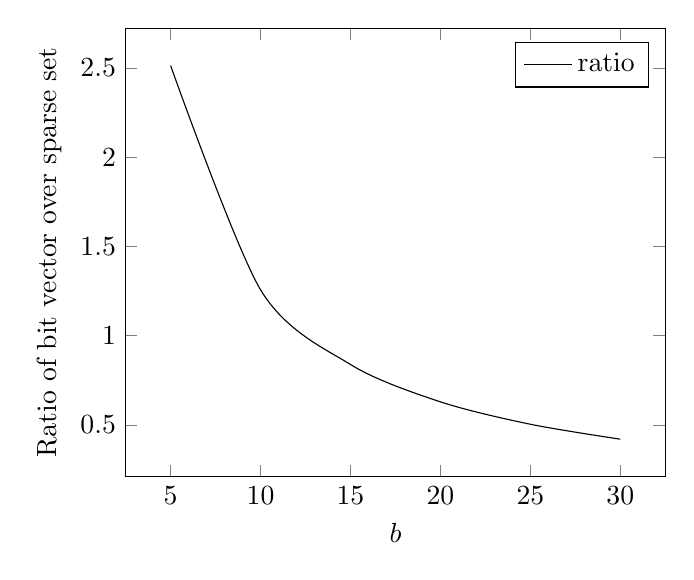
\begin{tikzpicture}
    \begin{axis}[
        legend pos=north east,
        xlabel=$b$,
        ylabel=Ratio of bit vector over sparse set]

        \addplot[black, smooth] plot coordinates {
            (5,  2.51302)
            (10, 1.25686)
            (15, 0.838169)
            (20, 0.628847)
            (25, 0.503276)
            (30, 0.419585)
        };

        \legend{ratio}
    \end{axis}
\end{tikzpicture}

\caption{The ratio of memory use of \texttt{bitset} over \texttt{set} as a
         function of $\beta$.}
\label{fig:bmem}
\end{figure}
Aside from the modifier set, we also have to store the set of variables that
are equal to zero in the optimal solutions of each subinstance. These sets
are more difficult to analyze in terms of memory use, simply because the
cardinality is unknown. However, we do know that $|\mathcal{Z}_k| \geq
|\mathcal{M}_k|$.

With sets of sparsely stored indices, we only need to check the variables
that are actually in the sets in order to determine if a set is a subset
of some set. However, with bit vectors, we need to check $n$ bits---where $n$
is the number of variables in the universe---in order to determine the same.
This means that the \texttt{isSubset} routine will most likely have a different
running time with the two implementations.

One way to find out which of the two are most suited for our need is to perform
a benchmark of the two.
By setting the universe to some size $n$, and generating sets of
random sparsity less than or equal to $n$, we can test how fast
\texttt{isSubset} will run.
We generate random sets as \texttt{bitsets} in \texttt{C++}, storing copies
of these sets in the sparse representation, then testing the performance 
of both implementations of \texttt{isSubset}.
Figure \ref{fig:setspeed}
shows the running time of the two implementations in seconds. Both
implementations were tested on $3000^2$ \texttt{isSubset}-executions, while
increasing $n$.
Codes for the benchmark can be found in Appendix \ref{app:setbench}.
\begin{figure}[ht!]
\centering
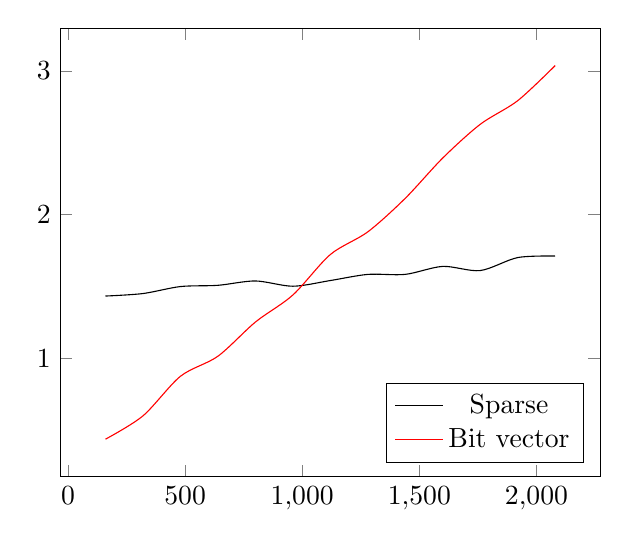
\begin{tikzpicture}
    \begin{axis}[
        legend pos=south east]
%        xlabel=Variables in Universe,
%        ylabel=Seconds]

        \addplot[black, smooth] plot coordinates {
(160, 1.43344)
(320, 1.45082)
(480, 1.49948)
(640, 1.50815)
(800, 1.53846)
(960, 1.50186)
(1120, 1.54138)
(1280, 1.58404)
(1440, 1.58431)
(1600, 1.63973)
(1760, 1.61084)
(1920, 1.70125)
(2080, 1.71173)
        };

        \addplot[red, smooth] plot coordinates {
(160, 0.437256)
(320, 0.599489)
(480, 0.875034)
(640, 1.01462)
(800, 1.25228)
(960, 1.44069)
(1120, 1.72237)
(1280, 1.88017)
(1440, 2.11386)
(1600, 2.39418)
(1760, 2.6287)
(1920, 2.79312)
(2080, 3.03735)
        };

        \legend{Sparse, Bit vector}
    \end{axis}
\end{tikzpicture}

\caption{CPU-seconds used to execute $3000^2$ calls to \texttt{isSubset} on
         randomly generated sets with random sparsity as a function of $n$.}
\label{fig:setspeed}
\end{figure}

We see that the bit vector implementation is much faster than the sparse
implementation on smaller universes. However, the sparse implementation
scales much better than the bit vector implementation when the size of
the universe increases. When it comes to memory, the situation is the same,
except reversed. The sets of sparsely stored indices obviously uses less
memory when $\beta$ is small, i.e. the modifiers are more sparse. However, they
do not scale as nicely as the bit vectors. So the choice relies on what is
most important: memory or speed. Since the nature of this thesis is to
implement a \emph{fast} solver, we give speed a higher priority than memory 
efficiency, so we choose to implement the sets of sparsely stored
indices. That is, in \texttt{C++}, \texttt{set}.

\subsection{Tree Construction}
Because we do not need to store any information about edges in the tree,
we do not need to implement edges as an object of its own. We defined
a vertex \texttt{struct} earlier, having a \texttt{vector} of child
vertices. That means that for each vertex we have, we can reach all child
vertices, children's child vertices and so on, from that vertex.
So, if we have a pointer to the root of a tree, we can reach all vertices
in the tree. Although we earlier defined a tree as an ordered pair
$(V, E)$ of a set of vertices $V$ and a set of edges $E$, we only need a
pointer \texttt{struct vertex*} to our root to access our tree.

The biggest operations in Algorithm \ref{alg:construct} is iterating the power
set of $\left\{1,2,\ldots,n\right\}$. There are lots of combination generators available, so
instead of re-inventing the wheel, we choose a generator that suits our needs.
We need one that is easy to use, and is capable of generating combinations of
a given cardinality. One implementation, similar in use to
\texttt{next\_permutation} in the standard \texttt{C++ STL}, is presented
in~\cite{codeproject}.
Codes from \cite{codeproject} can be found in Appendix
\ref{app:nextcombination}.

The remaining parts of the \texttt{construct}-routine is just running
\texttt{mfind} on each generated modifier, and adding it to the tree
if necessary. Then at the end, return the pointer to the root vertex.

\subsection{Discrete Event Simulation}
In a discrete event simulation (DES), operations are always triggered by events.
In a DES for the reliability analyses discussed in Chapter \ref{ch:intro},
we only need to consider two types of events; a breakdown in the network,
or that a link is repaired.
Each link in the network is represented by
a variable, so each event can by represented by a single variable.

The current state of our system is easily represented by a QP $\mathcal{Q}$ and
a set of variables representing the current broken links in our network.
As this set represents broken links, just like our modifiers $\mathcal{M}_k$
represents breakdowns, we choose to denote the current state of the system
by $\mathcal{M}$. 

Given a variable $x$ to represent a link that breaks down, we need to
update the  current state of the system. This is done with a simple
\textit{union}
\[
\mathcal{M} = \mathcal{M} \cup \left\{x\right\}.
\]
Given a variable $x$ of variables to represent a repaired link, we update the
current state with a simple \textit{relative complement}
\[
\mathcal{M} = \mathcal{M} \setminus \left\{x\right\}.
\]
We call these two operations for \texttt{break} and \texttt{repair}, respectively.
After every change of state in the system, we need to solve the subinstance
of $\mathcal{Q}$ defined by the modifier $\mathcal{M}$.

As the state of the system changes, we need to solve more and more subinstances.
We can choose whether or not we want to store the modifiers and their respective
solutions in a tree or not. If we choose to store distinct solutions in a tree,
we check the tree for a solution for the subinstance defined by the newly
updated modifier, before we potentially solve the problem.


\section{A Quick Overview}
In this section we present a quick overview of the different
implementations.

Although Clp is written primarily for solving linear
programs, it comes with a QP solver. This QP solver uses an implementation
of a primal-dual predictor-corrector interior point method. In addition
to Clp's QP solver, we also have the QP solver presented in Section
\ref{ch:slp}.

There are four different implementations we have, named
\texttt{construct\_clp}, \texttt{construct\_slp}, \texttt{naive\_clp} and
\texttt{naive\_slp}. The implementations with names ending with
\texttt{\_clp} and \texttt{\_slp} uses Clp's QP solver and Slp, respectively,
whenever a QP needs to be solved.
The \texttt{construct} implementations uses the tree structured presented
in Section \ref{ch:tree} for storing subinstances with distinct solutions.
The \texttt{naive} implementations, however, solves subinstances regardless of
whether they have distinct solutions or not.

In the next section, we present several experiments to perform on our
implementations.

%\endgroup

\chapter{Conclusion}
Goodtech and MathConsult have developed a tool called PROMAPS that calculates
the power delivery as a function of demand, and the probability for undelivered
energy for each load branch in the system, and in the system as a whole.
Among several main functions of PROMAPS, its bottleneck was pinpointed to
a call to a QP solver. The aim of this thesis was to improve the performance
of the methods initiated by this call.

We presented an iterative method based on linear programming, as the
presented data suggested that the QP problems were--- in lack of a better
word---\emph{close} to linear programs. Although this method turned out to be
slower than a commercially available alternate solver, due to the fact that the
number of iterations increases quite rapidly as the tolerance decreases, it
does stand as an alternative method, mainly because it does not require
any license fees.
It is important
to point out that the method is entirely independent of specific LP
implementations. The only requirement for implementing the method is an LP
solver. There are more available LP solvers than QP solvers in general,
but there are also more free LP solvers than free QP
solvers\cite{wikilp}\cite{wikiqp}.

Afterwards, we presented a tree structural approach for reducing the number
of calls to the QP solver. This approach reduced the number of calls to the
QP solver by a significant amount. Depending on problem size and the number
of breakdowns, this approach caused the original method to perform from
16\% to around 70\% faster, and we have reason to believe that it would
increase even further with $\beta$.
The tree structural approach therefore reduced the average number of
CPU-seconds used to solve a subinstance.
This method is
independent of the choice of QP solver, and since the method relies on reducing
the number of calls to the QP solver, and not increasing the speed of the
actual solver, the relative speedup will most likely remain solver independent.

\chapter{Future Work}
In this chapter, we present suggestions to future work regarding the methods
described in this thesis.

\section{Parallelization}
Since we are solving a huge amount of QP problems, running several QP solvers
in parallel is of interest. We suggest the parallelization of the methods
presented in this thesis as a future research topic.

%We consider the possibility of parallelizing both
%the naive method of solving all subinstances regardless of whether they are
%distinct or not, and the tree-structured approach. We begin by analyzing
%the parallelization of the naive approach.

If we are to parallelize the naive method on a distributed computer, we need to
analyze the amount of communication that is needed between processors.
Given some number of breakdowns $\beta$ and an instance $\mathcal{Q}$ with
$m$ rows and $n$ columns, we can map each subinstance of $\mathcal{Q}$ to some
$\mathcal{Q}_i$ for $i=0,1,\ldots,\sigma(\beta,n) - 1$. Each processor needs to
have a copy of the original instance $\mathcal{Q}$, which is $O(mn)$ in terms
of memory size. Given a number of processors $p$, the main processor needs to
transmit this problem to each processor, resulting in $O(pmn)$ in terms of
communication before the calculations are started. Now, each
processor solves $\frac{\sigma(\beta, n)}{p}$ subinstances, resulting in
\[
O(\sigma(\beta, n)n)
\]
in terms of communication by sending solutions back to the main processor.
Sending few, but huge blocks of data is often faster than sending many small
blocks of data.
Therefore, an alternative approach is to store all solutions on each processor,
and then transmitting them all to the main processor.
This would require
\[
O\left(\frac{\sigma(\beta, n)n}{p}\right)
\]
in terms of memory for each processor.

Further research topics may include parallelization of both the naive approach
and the tree structural approach on both a shared memory computer and a
distributed computer.

\section{Coordinate Descent}
Consider a minimization problem
\[
    \min f(x) = x^T H x + b^T x,
\]
where $H$ is diagonal a $n \times n$ matrix, and $x$ and $b$ are vectors in
$\mathbb{R}^n$.
Since $H$ is diagonal, the contours of $f$ are ellipses
whose axes are aligned with the coordinate directions\cite{nocedal}.
By performing successive one-dimensional minimizations along the
coordinate directions $e_1,e_2,\ldots,e_n$, we can find the minimizer of $f$
in $n$ iterations. This is illustrated in Figure \ref{fig:coordinatedescent}
for $n = 2$.

\begin{figure}[ht!]
\centering
\begin{tikzpicture}
    % grid and axes
    \draw[scale=1.5,->,name path=xaxis] (-0.2,0) -- (2.2,0) node[right] {$e_1$};
    \draw[scale=1.5,->,name path=yaxis] (0,-0.2) -- (0,2.2) node[above] {$e_2$};

    \draw[scale=1.5,fill] (qopt) circle [radius=0.02];

    \node at (0.25*1.5, 0.566987*1.5) (x0) {};
    \node at (1*1.5, 0.566987*1.5) (x1) {};
    \node at (1*1.5, 1*1.5) (x2) {};

    \draw[scale=1.5,fill] (x0) circle [radius=0.02];
    \draw[scale=1.5,fill] (x1) circle [radius=0.02];
    \draw[scale=1.5,fill] (x2) circle [radius=0.02];

    \draw[scale=1.5,-] (x0.center) -- (x1.center) -- (x2.center);

    % draw the quadratic objective function
    \draw[scale=1.5,thin, dashed] plot[id=qobj, raw gnuplot] function {
        f(x,y) = x**2 + y**2 - 2*x - 2*y + 1.25;
        set xrange[-1:2];
        set yrange[-2:2];
        set view 0,0;
        set isosamples 1000,1000;
        set size square;
        set cont base;
        set cntrparam levels incre 0,0.1,0;
        unset surface;
        splot f(x,y);
    };
    \draw[scale=1.5,thin, dashed] plot[id=qobj0, raw gnuplot] function {
        f(x,y) = x**2 + y**2 - 2*x - 2*y + 1.55;
        set xrange[-1:2];
        set yrange[-2:2];
        set view 0,0;
        set isosamples 1000,1000;
        set size square;
        set cont base;
        set cntrparam levels incre 0,0.1,0;
        unset surface;
        splot f(x,y);
    };
    \draw[scale=1.5,thin, dashed] plot[id=qobj1, raw gnuplot] function {
        f(x,y) = x**2 + y**2 - 2*x - 2*y + 1.75;
        set xrange[-1:2];
        set yrange[-2:2];
        set view 0,0;
        set isosamples 1000,1000;
        set size square;
        set cont base;
        set cntrparam levels incre 0,0.1,0;
        unset surface;
        splot f(x,y);
    };
    \draw[scale=1.5,thin, dashed] plot[id=qobj2, raw gnuplot] function {
        f(x,y) = x**2 + y**2 - 2*x - 2*y + 1.9;
        set xrange[-1:2];
        set yrange[-2:2];
        set view 0,0;
        set isosamples 1000,1000;
        set size square;
        set cont base;
        set cntrparam levels incre 0,0.1,0;
        unset surface;
        splot f(x,y);
    };
    \draw[scale=1.5,thin, dashed] plot[id=qobj3, raw gnuplot] function {
        f(x,y) = x**2 + y**2 - 2*x - 2*y + 1.98;
        set xrange[-1:2];
        set yrange[-2:2];
        set view 0,0;
        set isosamples 1000,1000;
        set size square;
        set cont base;
        set cntrparam levels incre 0,0.1,0;
        unset surface;
        splot f(x,y);
    };
\end{tikzpicture}

\caption{Illustration of minimization along the coordinate directions of a
         quadratic with a diagonal Hessian.}
\label{fig:coordinatedescent}
\end{figure}

We suggest the development of a direct method based upon coordinate
descent as a future research topic.

%\onecolumn
%\newpage
%\twocolumn

\bibliography{thesis}{}
\bibliographystyle{ieeetr}

\onecolumn
\appendix
\chapter{Example Tree of Some $\mathcal{Q}$}
\label{app:tree}
\centering
\begin{minipage}{0.49\linewidth}
\centering
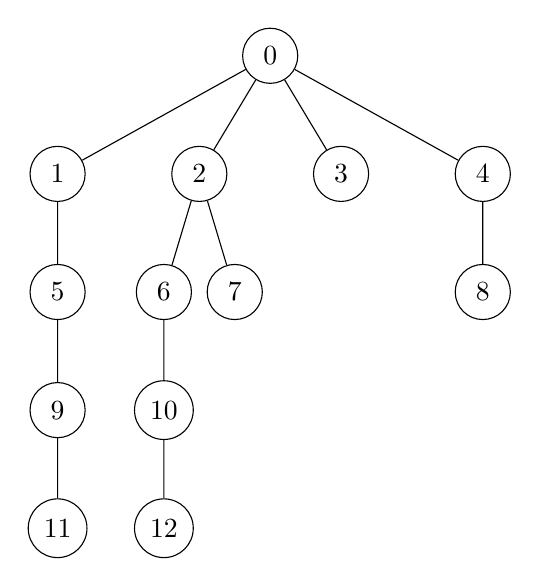
\begin{tikzpicture}[level/.style={sibling distance=18mm/#1}]
\tikzset{every node/.style={shape=circle,draw,minimum size=7mm}}
%\tikzset{every node/.style={shape=circle,
%                            font=\bfseries \Large,
%                            minimum size=3cm,
%                            scale=0.4
%                           }}
\node (root) {$0$}
    child {node (n1) {$1$}
        child {node (n5) {$5$}
            child {node (n9) {$9$}
                child {node (11) {$11$}
                }
            }
        }
    }
    child {node (n2) {$2$}
        child {node (n6) {$6$}
            child {node (n10) {$10$}
                child {node (n12) {$12$}
                }
            }
        }
        child {node (n7) {$7$}
        }
    }
    child {node (n3) {$3$}
    }
    child {node (n4) {$4$}
        child {node (n8) {$8$}
        }
    }
    ;
\end{tikzpicture}
\end{minipage}
\begin{minipage}{0.5\linewidth}
\centering
\begin{tabular}{rll}
         $k$ & $\mathcal{M}_k$            & $\mathcal{Z}_k$ \\ \hline
    0        & $\left\{{}\right\}$        & $\left\{{1,3}\right\}$ \\
    1        & $\left\{{2}\right\}$       & $\left\{{2,3,5}\right\}$ \\
    2        & $\left\{{4}\right\}$       & $\left\{{4,1,5}\right\}$ \\
    3        & $\left\{{5}\right\}$       & $\left\{{5,1,3}\right\}$ \\
    4        & $\left\{{2,4}\right\}$     & $\left\{{2,4,3,5}\right\}$ \\
    5        & $\left\{{2,1}\right\}$     & $\left\{{2,1,4,5}\right\}$ \\
    6        & $\left\{{4,3}\right\}$     & $\left\{{4,3,1}\right\}$ \\
    7        & $\left\{{4,2,3}\right\}$   & $\left\{{4,2,3,5}\right\}$ \\
    8        & $\left\{{2,4,1}\right\}$   & $\left\{{2,4,1,3}\right\}$ \\
    9        & $\left\{{2,1,3}\right\}$   & $\left\{{2,1,3,4}\right\}$ \\
    10       & $\left\{{4,3,5}\right\}$   & $\left\{{4,3,5,2}\right\}$ \\
    11       & $\left\{{2,1,3,5}\right\}$ & $\left\{{2,1,3,5}\right\}$ \\
    12       & $\left\{{4,3,5,1}\right\}$ & $\left\{{4,3,5,1,2}\right\}$
\end{tabular}
\end{minipage}


\chapter{Slp Header Files}

\section*{\texttt{Algorithm.hpp}}
\begin{verbatim}
/**
 * Perform a line search by finding the minimum objective value
 * of the given QP problem of all the points between the two
 * given points.
 *
 * @param  p1
 *         Start point.
 * @param  p2
 *         End point.
 * @param  model
 *         ClpModel of the QP problem.
 * @return the step length alpha.
 */
double lineSearch(double* p1, double* p2, const ClpModel model);
\end{verbatim}

\begin{verbatim}
/**
 * Solve a QP problem using Slp.
 *
 * @param  quad
 *         ClpModel containing the QP problem.
 * @param  x
 *         Array containing the initial guess vector. This array
 *         will be overwritten with a final solution.
 * @param  maxIters
 *         Number of iterations to perform if the stopping
 *         criteria is not met.
 * @param  tol
 *         Epsilon for the stopping criteria.
 * @return the objective value of the solved QP problem..
 */
double solve(ClpModel quad, double* x, int maxIters, double tol);
\end{verbatim}

\newpage

\begin{verbatim}
/**
 * Perform a Taylor-series expansion of the objective function of
 * the given QP problem at the given point.
 *
 * @param destCoeffs
 *        Pointer to coefficient destination.
 * @param point
 *        Point to perform the expansion at.
 * @param model
 *        ClpModel that has the objective function.
 */
void taylor(double* destCoeffs, double* point, ClpModel model);
\end{verbatim}

\begin{verbatim}
/**
 * Evaluate the objective function of the given model at
 * the given point.
 *
 * @param point
 *        Point to evaluate the objective function at.
 * @param model
 *        ClpModel that has the objective function to evaluate.
 */
doubld value(double* point, ClpModel model);
\end{verbatim}

\end{document}
